\documentclass{jknotes}
\usepackage{joshkirklin}

\begin{document}

\institution{Cambridge Part III Maths}
\title{Symmetries, Fields and Particles}
\lecturer{Nick Dorey}
\notetaker{Josh Kirklin}
\date{Michaelmas 2015}

\maketitle
\suggestionsspiel
\unlecturedspiel

\tableofcontents

\section{Introduction}

\subsection{Groups}

\begin{defn}
    A \emph{symmetry} is a transformation of a set of dynamical variables, under which the forms of all physical laws are invariant.
\end{defn}

\begin{eg}
    Consider rotations in 3D space: 
    \begin{equation}
        \vb{x} \in \RR^3 \mapsto \vb{x}' = M \cdot \vb{x} \in \RR^3
    \end{equation}
    Here, \(M\) is a \(3\times3\) real special orthogonal matrix:
    \begin{align}
        \det M &= 1 & \trans{M}M &= \identity
    \end{align}
    Newton's second law is invariant under these transformations, so rotations are a symmetry of Newtonian mechanics.
    \begin{equation}
        \vb{F} = m \vb{a} \longrightarrow \vb{F}' = m \vb{a}'
        \label{}
    \end{equation}
\end{eg}

Group theory provides us with a useful mathematical formulation of symmetries.

\begin{defn}
    A \emph{group} \((G,\cdot)\) is a set \(G\) equipped with a multiplication operator \(\cdot\) with the following properties:
    \begin{enumerate}[label=(\roman*)]
        \item \emph{Closure}: \(g_1,g_2 \in G \implies g_1\cdot g_2 \in G\)
        \item \emph{Identity}: \(\Exists e \in G \st e\cdot g = g = g\cdot e \Forall g \in G\)
        \item \emph{Inverses}: \(\Forall g \in G \Exists g^{-1} \in G \st g\cdot g^{-1} = g^{-1}\cdot g = e\)
        \item \emph{Associativity}: \(g_1\cdot (g_2\cdot g_3) = (g_1\cdot g_2)\cdot g_3 \Forall g_1, g_2, g_3 \in G\)
    \end{enumerate}
\end{defn}

The set in question may be either finite or infinite. We say that \((G,\cdot)\) is \emph{abelian} or \emph{commutative} if \(g_1\cdot g_2=g_2\cdot g_1 \Forall g_1, g_2 \in G\).

Often we will omit \(\cdot\) and just write \(G = (G,\cdot)\) and \(g_1g_2 = g_1 \cdot g_2\).

\begin{eg}
    Rotations in 3D space form a non-abelian group under composition\footnote{\emph{under} here being a way to specify the group operator.}. We call the group of \(3\times3\) real special orthogonal matrices \(SO(3)\). The elements of \(SO(3)\) depend on three parameters: \(\vu{n} \in S^2, \theta \in [0,\pi]\).
\end{eg}

\subsection{Manifolds}

\begin{defn}
    An \emph{\(n\)-manifold} is a space which locally looks like \(\RR^n\).
\end{defn}

\begin{eg}
    The 2-sphere $S^2$ is a 2-manifold.
\end{eg}

Let \(\mathcal{M}\) be a smooth manifold of dimension \(D\), and let \(p\) be a point in \(\mathcal{M}\). Since \(\mathcal{M}\) is locally like \(\RR^D\), we can introduce a set of coordinates \(\{x^i\}, i=1,\ldots,D\) into an open subset of the manifold, with origin at \(p\).

\begin{defn}
    The tangent space to \(\mathcal{M}\) at \(p\), denoted \(\mathcal{T}_p(\mathcal{M})\), is the \(D\)-dimensional vector space spanned by the differential operators \(\{\pdv{x^j}\}, j = 1,\ldots,D\).
    \begin{figure}[H]
        \centering
        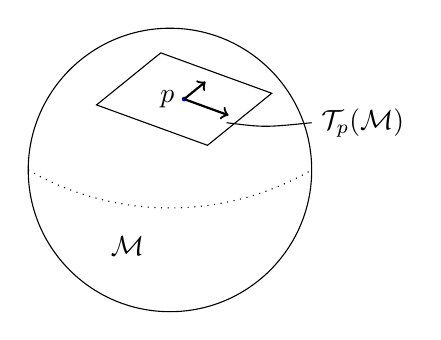
\begin{tikzpicture}[scale=0.6]
            \draw (0,0) circle (3);
            \draw[rotate=-90,dotted] (0,-3) arc (-30:30:6);
            \draw[-] (3,1) node[anchor=west] {\(\mathcal{T}_p(\mathcal{M})\)} .. controls (2,0.9) .. (1.2,1);
            \begin{scope}[shift={(0.3,1.5)}]
                \draw (0,0) node[anchor=east] {\(p\)};
                \fill[blue] (0,0) circle (0.05);
                \begin{scope}[rotate=-20,xslant=0.6]
                    \draw (-1.25,-0.75) rectangle (1.25,0.75);
                    \draw[->,thick] (0,0) -- (1,0);
                    \draw[->,thick] (0,0) -- (0,0.5);
                \end{scope}
            \end{scope}
            \draw (-0.9,-1.6) node {\(\mathcal{M}\)};
        \end{tikzpicture}
    \end{figure}
\end{defn}

Suppose \(f:\mathcal{M}\rightarrow\RR\) is a function on \(\mathcal{M}\), and let \(V=V^i\pdv{x^i} \in \mathcal{T}_p(\mathcal{M})\).
The action of \(V\) on \(f\) is defined as follows:
\begin{equation}
    V(f) = \left.V^i\pdv{f}{x^i}\right|_{x=0}
\end{equation}

Consider a smooth curve on \(\mathcal{M}\):
\begin{equation}
    \fullfunction{C}{\RR}{\mathcal{M}}{t}{x^i(t)}
\end{equation}
Suppose this curve goes through \(p\) at \(t=0\). We can associate a tangent vector at \(p\) with \(C\) in the following way:
\begin{equation}
    V_C = \dot{x}^i(0)\pdv{x^i} \in \mathcal{T}_p(\mathcal{M}) \text{ where } \dot{x}^i = \dv{x^i}{t}
\end{equation}
\begin{figure}[H]
    \centering
    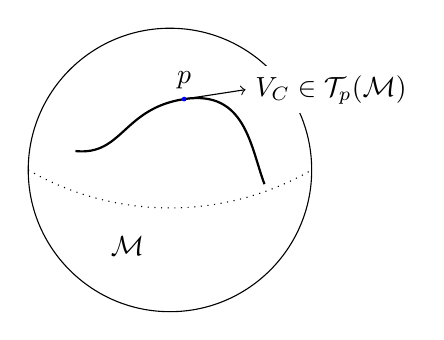
\begin{tikzpicture}[scale=0.6]
        \draw (0,0) circle (3);
        \draw[rotate=-90,dotted] (0,-3) arc (-30:30:6);
        \draw[thick] (-2,0.4) 
            .. controls (-1,0.3) and (-1,1.3) .. (0.3,1.5)
            .. controls (1.6,1.7) and (1.7,0.5) .. (2,-0.3);
        \draw[->] (0.3,1.5) -- (1.6,1.7) node[anchor=west,fill=white] {\(V_C \in \mathcal{T}_p(\mathcal{M})\)};
        \begin{scope}[shift={(0.3,1.5)}]
            \draw (0,0) node[anchor=south] {\(p\)};
            \fill[blue] (0,0) circle (0.05);
        \end{scope}
        \draw (-0.9,-1.6) node {\(\mathcal{M}\)};
    \end{tikzpicture}
\end{figure}
If we let \(V_C\) act on a function \(f\) we can see that it is simply the total derivative of \(f\) along the curve at \(p\):
\begin{equation}
    V_C(f) = \left.\dot{x}^i\pdv{x^i}f(x)\right|_{x=0} = \left.\dv{x^i}{t}\pdv{f}{x^i}\right|_{x=0} = \left.\dv{f}{t}\right|_p
\end{equation}
In physics, often \(C\) is the trajectory of a particle or other dynamical object, and \(V_C\) represents its velocity vector.

\subsection{Lie groups}

\begin{defn}
    A \emph{Lie group} \(G\) is a group which is also a smooth manifold. The group and manifold structures must be compatible, so for example the product \(\cdot : G \times G \rightarrow G\) and inverse operations must be smooth maps.
\end{defn}

We will see that \(G\) is (almost) completely determined by its behaviour ``near'' the identity \(e\).

We denote the manifold of \(G\) by \(\mathcal{M}(G)\). The dimension of \(G\), denoted \(\dim G\), is equivalent to the dimension of \(\mathcal{M}(G)\).

Let's introduce a set of coordinates \(\{\theta_i\}, i = 1, \ldots, D = \dim G\) in some local neighbourhood of the identity \(e \in G\), with \(e\) at the origin. The group elements in this neighbourhood depend continuously on the \(\{\theta_i\}\), and we can write \(g=g(\theta)\).

Multiplication of two of these elements corresponds to a smooth map \(G \times G \rightarrow G\):
\begin{equation}
    g(\theta)g(\theta^\prime) = g(\phi) \in G
\end{equation}

\subsection{Matrix groups}
Let \(\operatorname{Mat}_n(F)\) denote the set of \(n \times n\) matrices over a field \(F\). In these notes we will henceforth only consider \(F = \RR \text{ or } \CC\). Matrix multiplication is closed, associative, and there exists an identity, but \(\operatorname{Mat}_n(F)\) is \emph{not} a group under multiplication because not all elements have inverses.
The ``largest'' multiplicative group contained in \(\operatorname{Mat}_n(F)\) is the \emph{general linear group}, containing all invertible \(n\times n\) matrices:
\begin{equation}
    GL(n,F) = \{M\in \operatorname{Mat}_n(F) \st \det M \ne 0 \}
\end{equation}
If we require the determinant to be equal to 1, we obtain the \emph{special linear group}:
\begin{equation}
    SL(n,F) = \{M\in \operatorname{Mat}_n(F) \st \det M = 1 \}
\end{equation}
Note that the closure of and existence of inverses in \(SL(n,F)\) follows from the fact that multiplication commutes with taking the determinant, i.e. \(\det(M_1M_2) = \det M_1 \det M_2\).

We can see that these are groups; slightly less obviously they are also Lie groups.
\begin{align}
    \dim GL(n,\RR) &= n^2 & \dim GL(n,\CC) &= 2n^2 \\
    \dim SL(n,\RR) &= n^2 - 1 & \dim SL(n,\CC) &= 2n^2 - 1
\end{align}

\begin{defn}
    A \emph{subgroup} \(H\) of a group \(G\) is a subset of \(G\) which is also a group. If \(H\) is also a smooth submanifold, then we say that \(H\) is a \emph{Lie subgroup}.
\end{defn}

Of interest are the \emph{orthogonal groups}, which are subgroups of \(GL(n,\RR)\):
\begin{equation}
    O(n) = \{M \in GL(n,\RR) \st \trans{M}M = \identity\}
\end{equation}
Orthogonal transformations preserve the lengths of vectors.
\begin{equation}
    |\vb{v}'|^2 = \trans{\vb{v}'}\vb{v}' = \trans{\vb{v}}\trans{M}M\vb{v} = \trans{\vb{v}}\vb{v} = |\vb{v}|^2
\end{equation}
We also have \((\det M)^2 = \det (\trans{M} M) = \det \identity = 1\), so \(\det M = \pm 1\). The two cases correspond to the two connected components of \(O(n)\). Elements in the positive determinant component correspond to rotations in \(n\)-dimensional space, and elements in the negative determinat component correspond to a reflection composed with rotations. The fact that the identity does not contain a reflection allows us to define the \emph{special orthogonal groups}:
\begin{equation}
    SO(n) = \{M \in O(n) \st \det M = + 1 \}
\end{equation}
It can be checked that \(\dim O(n) = \dim SO(n) = \frac{1}{2}n(n+1)\).

It is easy to show that if \(\lambda\) is an eigenvalue of an orthogonal matrix \(M\), then we have the following:
\begin{enumerate}[label=(\roman*)]
    \item \(\lambda^*\) is also an eigenvalue of \(M\).
    \item \(|\lambda|^2 = 1\)
\end{enumerate}

\begin{eg}
    Let \(M \in SO(2)\). From the above, we can deduce that the eigenvalues of \(M\) are \(\lambda = e^{\pm i\theta}\) for some \(\theta \in \RR\), and we can write:
    \begin{equation}
        M(\theta) =
        \begin{pmatrix}
            \cos\theta & - \sin\theta \\
            \sin\theta & \cos\theta
        \end{pmatrix}
    \end{equation}
    These matrices are uniquely specified by \(\theta\) if we restrict \(0 \le \theta < 2\pi\). Since \(M(\theta) = M(\theta+2\pi)\), we can identify the manifold of \(SO(2)\) as the circle:
    \begin{equation}
        \mathcal{M}(SO(2)) \simeq S^1
    \end{equation}
\end{eg}

\begin{eg}
    Let \(M\in SO(3)\). From the above properties, we can see that the eigenvalues of \(M\) must be \(\lambda = 1, e^{\pm i\theta}\) for some \(\theta \in \RR\). Let \(\vu{n}\) be a normalised eigenvector for \(\lambda = 1\). We have \(M\vu{n}=\vu{n}\); \(\vu{n}\) is parallel to the axis of rotation of \(M\). It can be shown that a general group element of \(SO(3)\) can be written in the following form:
    \begin{equation}
        M(\vu{n},\theta)_{ij} = \cos\theta\delta_{ij} + (1 - \cos\theta)n_in_j - \sin\theta\epsilon_{ijk}n_k
    \end{equation}
    Note that \(M(\vu{n},2\pi-\theta) = M(-\vu{n},\theta)\). We can still specify all group elements if we restrict \(0 \le \theta \le \pi\). Note also that \(M(\vu{n},0) = \identity \Forall \vu{n}\).

    Consider \(\vb{w} = \theta \vu{n}\). Values of \(\vb{w}\) in the 3-ball of radius \(\pi\) specify the elements of \(SO(3)\).
    \begin{align}
        B_3 &= \{\vb{w} \in \RR^3 \st |\vb{w}| \le \pi\} \subset \RR^3
        &
        \partial B_3 &= \{\vb{w} \in \RR^3 \st |\vb{w}| = \pi\} \simeq S^2
    \end{align}
    If we identify \(\theta = \pi\) with \(\theta = - \pi\), then we uniquely specify points in \(SO(3)\). Hence, \(\mathcal{M}(SO(3))\) is defined from \(B_3\) by indentifying antipodal points on the boundary \(\partial B_3\).
    \begin{equation}
        \mathcal{M}(SO(3)) = B_3/\sim \text{ where } \vb{w} \sim \vb{w}' \iff \vb{w} = -\vb{w}' \text{ and } |\vb{w}| = \pi
    \end{equation}
    This manifold has the following properties:
    \begin{itemize}
        \item It has no boundary.
        \item It is connected (a path exists between any two points) but not simply connected (not all closed loops can contract to a point).
        \item Its fundamental group is equivalent to the integers mod 2: \(\Pi_1(SO(3)) = \ZZ_2\).
        \item It is compact (closed and bounded).
    \end{itemize}
\end{eg}

Note that the fact that orthogonal transformations preserve the lengths of vectors is equivalent to saying that they preserve the Euclidean metric on \(\RR^n\), i.e. \(g = \identity\). If we substitute the Euclidean metric for a more general metric of signature \((p,q)\):
\begin{equation}
    \eta = 
    \begin{pmatrix}
        \identity_p & 0 \\
        0 & -\identity_q
    \end{pmatrix}
\end{equation}
then we obtain the group \(O(p,q)\):
\begin{equation}
    O(p,q) = \{M\in GL(n,\RR) \st \trans{M}\eta M = \eta\}
\end{equation}

\begin{eg}
    The Lorentz group is \(O(3,1)\).
\end{eg}
These groups are non-compact.

If we replace \(\RR\) with \(\CC\) and transposition with Hermitian conjugation in the above, we can obtain the \emph{unitary groups}:
\begin{equation}
    U(n) = \{U\in GL(n,\CC) \st \herm{U}U = \identity\}
\end{equation}
Note that now, since the \(U\) are complex matrices, we have \(\det U) = e^{i\delta}\) where \(\delta \in \RR\). If we enforce that \(\det U = 1\), we obtain the \emph{special unitary groups}:
\begin{equation}
    SU(n) = \{U \in U(n) \st \det U = 1\}
\end{equation}

\begin{defn}
    Two Lie groups \(G\) and \(G'\) are \emph{isomorphic}, denoted \(G \simeq G'\), if there exists a bijective smooth map \(J\) from one group to the other, and this map preserves the group structure, i.e.:
    \begin{equation}
        J(g_1g_2) = J(g_1)J(g_2)
    \end{equation}
\end{defn}

\begin{eg}
    Let's examine \(U(1) = \{z \in \CC \st |z|^2 = 1\}\). From this definition we see that elements in \(U(1)\) take the form \(z = e^{i\theta}, \theta \in [0,2\pi)\), and we can immediately observe that \(U(1) \simeq SO(2)\), with isomorphism function given by:
    \begin{equation}
        e^{i\theta} \mapsto 
        \begin{pmatrix}
            \cos\theta & -\sin\theta\\
            \sin\theta & \cos\theta
        \end{pmatrix}
    \end{equation}
\end{eg}

\begin{eg}
    It can be shown that a general form for all \(U \in SU(2)\) is:
    \begin{equation}
        U = a_0\identity + i \vb{a}\cdot\vb{\sigma}
    \end{equation}
    where the \(\sigma_i, i = 1,2,3\) are the Pauli matrices. Importantly, we must have \(a_0^2 + a_1^2 + a_2^2 + a_3^2 = 1\), which shows that \(\mathcal{M}(SU(2)) = S^3\).
\end{eg}

\subsection{Lie algebras}
\begin{defn}
    A \emph{Lie algebra} \(\mathfrak{g}\) is a vector space over a field \(F\), equipped with a \emph{bracket} \([\;,\;]:\mathfrak{g}\times\mathfrak{g}\rightarrow\mathfrak{g}\) with the following properties:
    \begin{enumerate}[label=(\roman*)]
        \item \emph{Anti-symmetry}: \([X,Y] = -[Y,X]\)
        \item \emph{Linearity}: \([\alpha X + \beta Y, Z] = \alpha[X,Z] + \beta[Y,Z]\)
        \item \emph{Jacobi identity}: \([X,[Y,Z]] + [Y,[Z,X]] + [Z,[X,Y]] = 0\)
    \end{enumerate}
\end{defn}

\begin{eg}
    If a vector space \(V\) has an associative linear product \(*\), then we can get a Lie algebra by setting:
    \begin{equation}
        [X,Y] = X*Y-Y*X
    \end{equation}
    This bracket is known as the \emph{commutator}. The commutator can provide lots of examples of Lie algebras. For example, we can let \(V\) be a vector space of matrices, and let \(*\) be matrix multiplication.
\end{eg}

The dimension of a Lie algebra \(\mathfrak{g}\), denoted \(\dim \mathfrak{g}\), is given by the dimension of its vector space.

If we choose a basis \(\{T^a\}\), where \(a = 1, \ldots, n = \dim \mathfrak{g}\), we can expand any \(X \in \mathfrak{g}\) in terms of its components:
\begin{equation}
    X = X_aT^a
\end{equation}
\begin{defn}
    If we apply the bracket to any two basis vectors, we obtain the \emph{structure constants} \(f_c^{ab}\):
    \begin{equation}
        [T^a,T^b] = f_c^{ab}T^c
    \end{equation}
\end{defn}
Note that the structure constants are dependent on the basis chosen. From the properties of the bracket, the structure constants obey the following:
\begin{align}
    f_c^{ab} = -f_c^{ba}\\
    f_c^{[ab}f_e^{d]c} = 0
\end{align}

\begin{defn}
    Two Lie algebras \(\mathfrak{g}\) and \(\mathfrak{g}'\) are \emph{isomorphic} if there exists a bijective linear map \(f:\mathfrak{g}\rightarrow\mathfrak{g}'\) that preserves the bracket:
    \begin{equation}
        [f(X),f(Y)] = f([X,Y])
    \end{equation}
\end{defn}
We are concerned with classifying Lie algebras up to isomorphism.

\begin{defn}
    A \emph{subalgebra} \(\mathfrak{h} \subset \mathfrak{g}\) is a subset which is also a Lie algebra.
\end{defn}
\begin{defn}
    An \emph{ideal} \(\mathfrak{h}\) of \(\mathfrak{g}\) is a subalgebra such that \([X,Y]\in\mathfrak{h} \Forall X\in\mathfrak{g},Y\in\mathfrak{h}\).
\end{defn}
\begin{eg}
    Every Lie algebra \(\mathfrak{g}\) has two \emph{trivial} ideals:
    \begin{equation}
        \mathfrak{h} = \{0\}, \mathfrak{h} = \mathfrak{g}
    \end{equation}
\end{eg}
\begin{eg}
    The \emph{derived algebra}:
    \begin{equation}
        \mathfrak{i}(\mathfrak{g}) = \{[X,Y] \st X,Y \in \mathfrak{g}\}
    \end{equation}
    is an ideal.
\end{eg}
\begin{eg}
    The \emph{center}:
    \begin{equation}
        J(\mathfrak{g}) = \{X \in \mathfrak{g} \st [X,Y] = 0 \Forall Y \in \mathfrak{g}\}
    \end{equation}
    is an ideal.
\end{eg}

\begin{defn}
    A Lie algebra is said to be \emph{abelian} if its bracket is always equal to \(0\).
\end{defn}
If \(\mathfrak{g}\) is abelian, then \(\mathfrak{i}(\mathfrak{g}) = \{0\}\) and \(J(\mathfrak{g}) = \mathfrak{g}\).

\begin{defn}
    A Lie algebra \(\mathfrak{g}\) is said to be \emph{simple} if it is non-abelian and has no non-trivial ideals.
\end{defn}
If \(\mathfrak{g}\) is simple, then \(\mathfrak{i}(\mathfrak{g}) = \mathfrak{g}\) and  \(J(\mathfrak{g}) = \{0\}\).

\section{Lie algebras from Lie groups}

\subsection{\texorpdfstring{${\cal L}(G)$}{L(G)}}

Let \(G\) be a Lie group of dimension \(D\) and introduce coordinates \(\{\theta^i\},i=1,\ldots,D\) in a region containing the identity \(e\) at \(\theta=0\). We have that \(\mathcal{T}_e(G)\) is a vector space of dimension \(D\). We will define a bracket \([\;,\;]:\mathcal{T}_e(G)\times\mathcal{T}_e(G)\rightarrow\mathcal{T}_e(G)\) which will show that \(\mathcal{L}(G) = (\mathcal{T}_e(G),[\;,\;])\) is a Lie algebra.

This is easiest do for matrix Lie groups \(G \subset \operatorname{Mat}_n(F)\). We can map tangent vectors to matrices:
\begin{equation}
    \mathcal{T}_e(G) \ni v^i\pdv{\theta^i} \mapsto \left.v^i\pdv{g(\theta)}{\theta^i}\right|_{\theta=0} \in \operatorname{Mat}_n(F)
\end{equation}
With this mapping we identify \(\mathcal{T}_e(G)\) with the subspace of \(\operatorname{Mat}_n(F)\) spanned by \(\{\pdv{g(\theta)}{\theta^i}\},i=1,\ldots,D\). Now we can define the obvious bracket, the \emph{matrix commutator}:
\begin{equation}
    [X,Y] = XY-YX
\end{equation}
This obeys most of the properties of a Lie bracket. The only one that is slightly non-trivial is that the Lie algebra is closed under the bracket, i.e. \([X,Y] \in \operatorname{span}\{\pdv{g(\theta)}{\theta^i}\}\). We will show this now.

To do so we use the correspondence between curves and tangent vectors shown earlier. Suppose \(C\) is a curve with that passes through the identity \(e\) with tangent vector \(X \in \mathcal{T}_e(G)=\mathcal{L}(G)\):
\begin{align}
    C:t &\mapsto g(t) \in G & g(0) &=e=\identity
\end{align}
Since \(\left.\dv{g(t)}{t}\right|_{t=0}\), we can expand \(g(t)\) as a Taylor series near \(t=0\) in the following way:
\begin{equation}
    g(t) = \identity + tX + O(t^2)
\end{equation}
Now suppose we have two elements \(X_1,X_2 \in \mathcal{L}(G)\) and corresponding curves \(C_1,C_2\):
\begin{align}
    C_1:t &\mapsto g_1(t) \in G & g_1(0)=g_2&(0)=\identity\\
    C_2:t &\mapsto g_2(t) \in G & \dot{g}_1(0)=X_1,&\;\dot{g}_2(0)=X_2
\end{align}
Now expanding to second order, we can write:
\begin{align}
    g_1(t) &= \identity + X_1t + W_1t^2 + O(t^3)\\
    g_2(t) &= \identity + X_2t + W_2t^2 + O(t^3)
\end{align}
for some \(W_1,W_2 \in \operatorname{Mat}_n(F)\). In order to show that \(\mathcal{L}(G)\) is closed, we need to find a new curve with tangent vector \([X_1,X_2]\). To that end, let us define \(h(t) = g_1^{-1}(t)g_2^{-1}(t)g_1(t)g_2(t)\). Obviously \(h(0) = \identity\), so we can set \(h(t) = \identity + h_1t + h_2t^2 + O(t^3)\). If we evaluate \(g_2(t)g_1(t)h(t) = g_1(t)g_2(t)\) term by term, we find that \(W_1,W_2\) cancel from our equations and we obtain:
\begin{equation}
    h_1 = 0, h_2 = [X_1,X_2]
\end{equation}
So define a new curve \(C_3\):
\begin{equation}
    C_3 : s \mapsto g_3(s) = h(\sqrt{s}) \in G
\end{equation}
We have:
\begin{equation}
    g_3(s) = \identity + s[X_1,X_2] + O(s^{3/2})
\end{equation}
Thus the tangent vector to this curve at the identity is \([X_1,X_2]\). So we have shown that \([X_1,X_2] \in \mathcal{L}(G)\) and thus that \(\mathcal{L}(G)\) is closed. Therefore, \(\mathcal{L}(G)\) is a real\footnote{That is, it has real structure constants} Lie algebra of dimension \(D\).

\begin{eg}
    Consider \(G=SO(2)\). A curve on \(G\) can be written:
    \begin{equation}
        g(t)=g(\theta(t))=
        \begin{pmatrix}
            \cos\theta(t) & -\sin\theta(t) \\
            \sin\theta(t) & \cos\theta(t)
        \end{pmatrix}
    \end{equation}
    \begin{equation}
        \implies \dot{g}(0)=
        \begin{pmatrix}
            0 & -1 \\
            1 & 0
        \end{pmatrix}
        \dot{\theta}(0)
    \end{equation}
    where we have assumed \(g(0)=\identity\). Therefore we can deduce the Lie algebra associated with \(G\):
    \begin{equation}
        \mathcal{L}(SO(2)) = \left\{ 
        \begin{pmatrix}
            0 & -c \\
            c & 0
        \end{pmatrix},
        c \in \RR
        \right\}
    \end{equation}
\end{eg}

\begin{eg}
    More generally, consider \(G=SO(n)\) or \(O(n)\), and let \(g(t)=R(t)\) be a curve in \(G\) that goes through the identity at \(t=0\). We have:
    \begin{equation}
        \trans{R}(t)R(t) = \identity
    \end{equation}
    Differentiating both sides with respect to \(t\) gives:
    \begin{equation}
        \trans{\dot{R}}(t) R(t) + \trans{R}(t) \dot{R}(t) = 0
    \end{equation}
    If we now set \(t=0\), and use \(R(0)=\identity\), we obtain:
    \begin{equation}
        \trans{X} + X = 0
    \end{equation}
    where \(\dot{R}(0) = X \in \mathcal{L}(G)\). In other words, \(X\) is antisymmetric. Hence:
    \begin{equation}
        \mathcal{L}(SO(n))=\mathcal{L}(O(n))=\{X\in\operatorname{Mat}_n(\RR)\st\trans{X}=-X\}
    \end{equation}
    By examining the number of independent components in an antisymmetric matrix, we can deduce that \(\dim G=\frac{1}{2}n(n-1)\).
\end{eg}

\begin{eg}
    Consider \(G=SU(n)\). As before let \(g(t)=U(t)\in SU(n)\) with \(U(0)=\identity\).
    \begin{equation}
        \herm{U}(t)U(t)=\identity \implies \herm{Z}+Z=0
    \end{equation}
    where \(Z=\dot{U}(0)\), i.e. \(Z\) is anti-Hermitian. But we have another constraint that will be relevant:
    \begin{equation}
        \det U(t) = 1
    \end{equation}
    Let's Taylor expand near \(t=0\):
    \begin{align}
        U(t) &= \identity + tZ + O(t^2) \\
        \implies \det U(t) &= 1 + \tr Z t + O(t^2)
    \end{align}
    Thus we must have \(\tr Z = 0\). Therefore:
    \begin{equation}
        \mathcal{L}(SU(n)) = \{Z \in \operatorname{Mat}_n(\CC) \st \herm{Z}=-Z, \tr Z = 0\}
    \end{equation}
    There are \(2n^2-n^2 - 1 = n^2-1\) independent components of a traceless anti-Hermitian complex matrix, so we have \(\dim G = n^2 - 1\).
\end{eg}
We did not consider the \(\det R = 1\) case for \(\mathcal{L}(SO(n))\), but if we had we would have again obtained that \(\tr R = 0\). Note however that \(R\) being antisymmetric implies that \(R\) is traceless, so we do not need to additionally specify this.
\begin{eg}
    From above, we have \(\mathcal{L}(SU(2))=\{2\times2\text{ traceless anti-Hermitian matrices}\}\). Consider the Pauli matrices:
    \begin{align}
        \sigma_1 &=
        \begin{pmatrix}
            0 & 1 \\
            1 & 0
        \end{pmatrix}
        &
        \sigma_2 &=
        \begin{pmatrix}
            0 & -i \\
            i & 0
        \end{pmatrix}
        &
        \sigma_3 &=
        \begin{pmatrix}
            1 & 0 \\
            0 & -1
        \end{pmatrix}
    \end{align}
    These are traceless and Hermitian. Thus we can choose the following basis for for \(\mathcal{L}(G)\):
    \begin{equation}
        T^a = -\frac{1}{2}i\sigma_a
    \end{equation}
    where the factor of \(-\frac{1}{2}\) is for future convenience. The Pauli matrices obey the following convenient identity:
    \begin{equation}
        \sigma_a\sigma_b = \delta_{ab}\identity + i\epsilon_{abc}\sigma_c
    \end{equation}
    With this we can calculate the bracket of any two basis elements:
    \begin{equation}
        [T^a,T^b] = -\frac{1}{2}[\sigma_a,\sigma_b] = -\frac{1}{2}i\epsilon_{abc}\sigma_c = \epsilon_{abc}T^c
    \end{equation}
    So the structure constants are \(f^{ab}_c = \epsilon_{abc}\).
\end{eg}
\begin{eg}
    We have \(\mathcal{L}(SO(3)) = \{3\times3\text{ real antisymmetric matrices}\}\). It is convenient to choose the following basis:
    \begin{align}
        T^1 &=
        \begin{pmatrix}
            0 & 0 & 0 \\
            0 & 0 & -1 \\
            0 & 1 & 0
        \end{pmatrix}
        &
        T^2 &=
        \begin{pmatrix}
            0 & 0 & 1 \\
            0 & 0 & 0 \\
            -1 & 0 & 0
        \end{pmatrix}
        &
        T^3 &=
        \begin{pmatrix}
            0 & -1 & 0 \\
            1 & 0 & 0 \\
            0 & 0 & 0
        \end{pmatrix}
    \end{align}
    The reason this basis is convenient is that we can write \((T^a)_{bc} = -\epsilon_{abc}\). It is not difficult to then show that \([T^a,T^b] = \epsilon_{abc}T^c\), so the structure constants are \(f^{ab}_c = \epsilon_{abc}\).
\end{eg}
Since we can choose bases in which \(SO(3)\) has the same structure constants as \(SU(2)\), we have \(\mathcal{L}(SO(3))\simeq\mathcal{L}(SU(2))\), despite the fact that \(SO(3)\not\simeq SU(2)\).

\subsection{Natural maps on Lie groups}
\begin{defn}
    Let \(G\) be a Lie group. For each \(h \in G\) we have two smooth maps \(L_h,R_h\), called \emph{left translation} and \emph{right translation} respectively:
    \begin{align}
        \fullfunction{L_h}{G}{G}{g}{hg}&
        &
        \fullfunction{R_h}{G}{G}{g}{gh}&
    \end{align}
\end{defn}
In what follows we will focus on \(L_h\), but similar results apply for \(R_h\).
\begin{lemma}
    \(L_h\) is a diffeomorphism\footnote{i.e. a smooth bijection with a smooth inverse.}.
\end{lemma}
\begin{proof}
    We have \(L_h(h^{-1}g)=g\) for all \(g \in G\), so \(L_h\) is surjective. Suppose \(g,g'\in G\) and \(L_h(g)=L_h(g')\). Then \(hg=hg'\implies g=g'\), so \(L_h\) is injective. Thus \(L_h\) is a bijection, and since it is defined as a product of two Lie group elements, it is a smooth one. Furthermore, we have that the inverse map \((L_h)^{-1}=L_{h^{-1}}\) is also smooth.
\end{proof}
Here we will sketch the consequences of this proposition. Introduce a set of coordinates \(\{\theta^i\}, i=1,\ldots,D\), with \(e\) at \(\theta=0\). Let \(g=g(\theta)\in G\) and \(g'=g(\theta')=L_h(g)=hg(\theta)\). From this we see that \(L_h\) is specified by \(\theta'^i=\theta'^i(\theta)\). Since \(L_h\) is a diffeomorphism, the Jacobian matrix exists:
\begin{equation}
    J_j^i(\theta) = \pdv{\theta'^i}{\theta^j}
\end{equation}
and it must be invertible, i.e. \(\det J\ne0\).

Left translation \(L_h\) induces a map \(L_h^*\) from tangent vectors at \(g\in G\) to tangent vectors at \(L_h(g) = hg \in G\).
\begin{figure}[H]
    \centering
    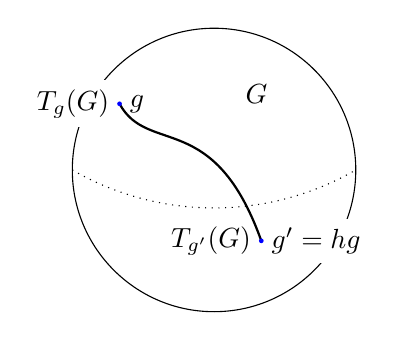
\begin{tikzpicture}[scale=0.6]
        \draw (0,0) circle (3);
        \draw[rotate=-90,dotted] (0,-3) arc (-30:30:6);
        \draw[thick] (-2,1.4) 
            node[anchor=east,fill=white] {\(T_g(G)\)}
            node[anchor=west] {\(g\)}
            .. controls (-1.4,0.3) and (0,1.3) .. (1,-1.5)
            node[anchor=east] {\(T_{g'}(G)\)}
            node[anchor=west,fill=white] {\(g'=hg\)};
        \fill[blue] (-2,1.4) circle (0.05);
        \fill[blue] (1,-1.5) circle (0.05);
        \draw (0.9,1.6) node {\(G\)};
    \end{tikzpicture}
\end{figure}
We define this map in the following way:
\begin{equation}
    \fullfunction{L_h^*}{\mathcal{T}_g(G)}{\mathcal{T}_{hg}(G)}{V=V^i\pdv{\theta^i}}{V'=V'^i\pdv{\theta'^i}}
    \text{ where }
    V'^i = J^i_j(\theta)V^j
\end{equation}

\begin{defn}
    A \emph{vector field} \(V\) assigns a tangent vector to each point \(g \in G\):
    \begin{equation}
        V(g) \in \mathcal{T}_g(G)
    \end{equation}
\end{defn}
Starting with a non-zero tangent vector at the identity \(W \in \mathcal{T}_e(G)\), we can define a vector field by:
\begin{equation}
    V(g) = L_g^*(W)
\end{equation}
This vector field is smooth, and since \(J\) is invertible it is non-vanishing. So if we start with a basis \(\{W_a\}, a=1,\ldots,D\) of the tangent space at the identity, then we obtain \(D\) independent non-vansishing vector fields \(V_a(g)=L_g^*(W_a)\). Although it may not seem so at first, the presence of these vector fields is a very strong constraint.
\begin{eg}
    The so-called ``Hairy ball theorem'' says that a smooth vector field defined on \(S^2\) must have at least one zero. Thus we cannot have a Lie group whose underlying manifold is the 2-sphere. So suppose \(G\) is a compact Lie group of dimension 2. Then we must have \(G=T^2=S^1\times S^1\), and \(G \simeq U(1)\times U(1)\). This is the only Lie group of dimension 2.
\end{eg}

Now consider matrix Lie groups.

\begin{lemma}
    Suppose we have a matrix Lie group \(G \subset \operatorname{Mat}_n(F)\), and \(h\in G, X \in \mathcal{L}(G)\). Then \(L_h^*(X) = hX \in \mathcal{T}_h(G)\).
\end{lemma}
\begin{proof}
    Let \(C\) be a curve with tangent vector \(X\) at the identity:
    \begin{align}
        \fullfunction{C}{\RR}{G}{t}{g(t)} && g(0)=e && \dot{g}(0) = X
    \end{align}
    Near \(t=0\) we can write:
    \begin{equation}
        g(t)=\identity+tX+O(t^2)
    \end{equation}
    Now define a new curve:
    \begin{align}
        \fullfunction{C_1}{\RR}{G}{t}{h(t)=hg(t)}
    \end{align}
    We have \(h(0)=h\) and \(\dot{h}(0)=h\dot{g}(0)=hX\), and hence near \(t=0\):
    \begin{equation}
        h(t) = h + thX + O(t^2)
    \end{equation}
    Thus \(hX \in \mathcal{T}_h(G)\).
\end{proof}
\begin{cor}
    Given some smooth curve in \(G\):
    \begin{align}
        \fullfunction{C}{\RR}{G}{t}{g(t)} && \dot{g}(t) \in \mathcal{T}_{g(t)}(G)
    \end{align}
    we can deduce that:
    \begin{equation}
        g^{-1}(t)\dot{g}(t) = L_{g^{-1}(t)}^*(\dot{g}(t)) \in \mathcal{T}_e(G) = \mathcal{L}(G)
    \end{equation}
\end{cor}
Conversely, given \(X \in \mathcal{L}(G)\), the following yields a curve in \(G\):
\begin{align}
    g^{-1}(t)\dot{g}(t) = X && g(0) = \identity \tag{\(*\)}
    \label{eqn:tangenttocurve}
\end{align}
\begin{defn}
    The \emph{exponential} of a matrix \(M\in \operatorname{Mat}_n(F)\) is given by the following:
    \begin{equation}
        \Exp M = \sum_{l=0}^\infty \frac{1}{l!}M^l \in \operatorname{Mat}_n(F)
    \end{equation}
\end{defn}

We can solve \eqref{eqn:tangenttocurve} by setting \(g(t)=\Exp(tX)\).
\begin{proof}
    We immediately have \(g(0)=\Exp(0)=\identity\). Also:
    \begin{align}
        g(t) &= \Exp(tX) = \sum_{l=0}^\infty\frac{1}{l!}t^lX^l\\
        \implies \dot{g}(t) &= X \left( \sum_{l=0}^\infty\frac{1}{l!}t^lX^l \right) = \Exp(tX)X = g(t)X\\
        \implies g^{-1}(t)\dot{g}(t)&=X
    \end{align}
\end{proof}

A useful identity that holds for all \(X \in \operatorname{Mat}_n(F)\) is:
\begin{equation}
    \det(\Exp X) = \exp(\tr(X))
\end{equation}

\begin{lemma}
    With a suitable choice of range \(J\) the set \(S_{X,J} = \{g(t) = \Exp(tX) \Forall t \in J \subset \RR\}\) is an abelian Lie subgroup of \(G\) with dimension 1, and \(S_{X,J}\simeq U(1)\) or \((\RR,+)\).
\end{lemma}
\begin{proof} (sketch)
    We have:
    \begin{equation}
        g(t_1)(t_2) = g(t_1+t_2) = g(t_2)g(t_1)
    \end{equation}
    so \(S_{X,J}\) is abelian and closed. Also we have an identity \(g(0) = \identity\) and inverses \((g(t))^{-1} = g(-t)\). Associativity is inherited.
    Now there are two cases to consider:
    \begin{enumerate}
        \item Compact case: there is some value of \(t_1 \ne 0\) such that \(g(t_1) = \identity\). Choose the least such \(t_1\) and set \(J = [0,t_1)\). 
                \begin{figure}[H]
                    \centering
                    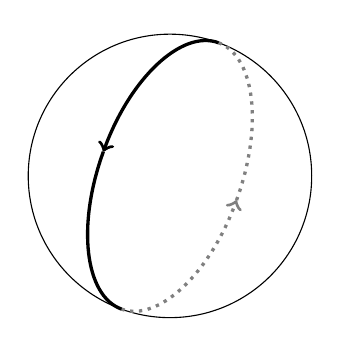
\begin{tikzpicture}[scale=0.6]
                        \draw (0,0) circle (3);
                        \begin{scope}[rotate=250,yscale=0.5, very thick]
                            \draw[dotted,->,gray] (3,0) arc (0:90:3);
                            \draw[dotted, gray] (0,3) arc (90:180:3);
                            \draw[->] (-3,0) arc (180:270:3);
                            \draw (0,-3) arc (270:360:3);
                        \end{scope}
                    \end{tikzpicture}
                \end{figure}
                Then we see that \(S_{X,J} \simeq U(1)\) with isomorphism \(g(t) \mapsto \exp(2\pi i t/t_1)\).
        \item Non-compact case: for all \(t \ne 0\), \(g(t) \ne \identity\). Then set \(J = \RR\), and we see that \(S_{X,J} \simeq (\RR,+)\) with isomorphism \(g(t) \mapsto t\).
                \begin{figure}[H]
                    \centering
                    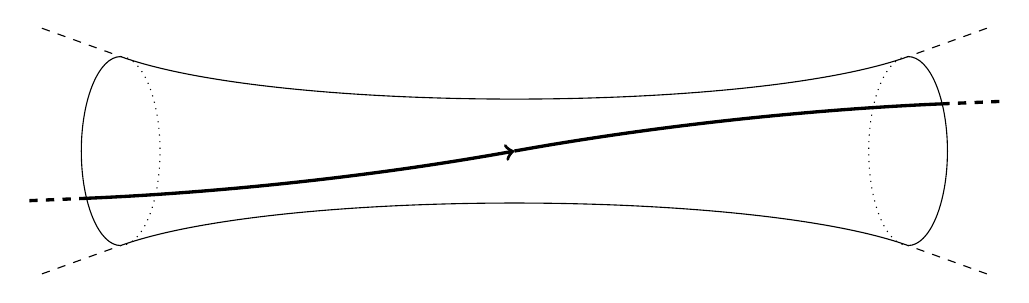
\begin{tikzpicture}[yscale=0.6]
                        \begin{scope}[dashed]
                            \draw (-6,-2.6) -- (-5,-2);
                            \draw (6,-2.6) -- (5,-2);
                            \draw (-6,2.6) -- (-5,2);
                            \draw (6,2.6) -- (5,2);
                        \end{scope}
                        \draw (-5,2) .. controls (-3,0.8) and (3,0.8) .. (5,2);
                        \draw (-5,-2) .. controls (-3,-0.8) and (3,-0.8) .. (5,-2);
                        \begin{scope}[shift={(5,0)},xscale=0.25]
                            \draw (0,2) arc (90:-90:2);
                            \draw[dotted] (0,2) arc (90:270:2);
                        \end{scope}
                        \begin{scope}[shift={(-5,0)},xscale=0.25]
                            \draw[dotted] (0,2) arc (90:-90:2);
                            \draw (0,2) arc (90:270:2);
                        \end{scope}
                        \draw[very thick,dashed] (-6.16,-1.05) -- (-5.44,-1);
                        \draw[very thick,->] (-5.44,-1) .. controls (-4,-0.9) and (-2,-0.6) .. (0,0);
                        \draw[very thick] (0,0) .. controls (2,0.6) and (4,0.9) .. (5.44,1);
                        \draw[very thick,dashed] (6.16,1.05) -- (5.44,1);
                    \end{tikzpicture}
                \end{figure}
    \end{enumerate}
\end{proof}

\subsection{Reconstructing \texorpdfstring{$G$}{G} from \texorpdfstring{${\cal L}(G)$}{L(G)}}
\begin{defn}
    Setting \(t=1\) defines the \emph{exponential map}:
    \begin{equation}
        \fullfunction{\operatorname{Exp}}{\mathcal{L}(G)}{G}{X}{\Exp{X}}
    \end{equation}
\end{defn}
Although we will not prove it here, in some neighbourhood of the identity, \(\Exp\) is a bijective map. So, given some \(X, Y \in \mathcal{L}(G)\), we have \(g_X=\Exp(X),g_Y=\Exp(Y) \in G\), and we expect \(g_Xg_Y=g_Z=\Exp(Z)\) for some \(Z \in \mathcal{L}(G)\). \(Z\) is determined using the \emph{Baker-Campbell-Haussdorf formula}:
\begin{equation}
    \Exp(X)\Exp(Y)=\Exp(Z)
    \implies
    Z = X + Y + \frac{1}{2}[X,Y] + \frac{1}{12}\left( [X,[X,Y]] - [Y,[X,Y]] \right) + \cdots
    \tag{BCH}
    \label{BCH}
\end{equation}

So \(\mathcal{L}\) completely determines \(G\) in some neighbourhood of the identity. 

Note that \(\Exp\) is not globally bijective; in particular:
\begin{itemize}
    \item It is not surjective when \(G\) is disconnected.
    \item It is not injective when \(G\) has a \(U(1)\) subgroup.
\end{itemize}

\begin{eg}
    Consider \(G=O(n)\). We have shown above that:
    \begin{equation}
        \mathcal{L}(O(n))=\{X\in\operatorname{Mat}_n(\RR)\st\trans{X}=-X\}
    \end{equation}
    \(X\) being antisymmetric implies that it is traceless, and hence that \(\det(\Exp X)=\exp(\tr X) = 1\). Therefore \(\Exp(X) \in SO(n)\subsetneqq O(n)\), so \(\Exp\) is not surjective.
\end{eg}
More generally, the image of \(\mathcal{L}(G)\) under \(\Exp\) is the connected component of the identity in \(G\).
\begin{eg}
    Consider \(G=U(1)\). We have \(\mathcal{L}(G) = \mathbb{I}\), the imaginary numbers. But then \(\Exp x = \Exp(x+2\pi i)\), so \(\Exp\) is not injective.
\end{eg}

\subsection{\texorpdfstring{$SU(2)$}{SU(2)} vs \texorpdfstring{$SO(3)$}{SO(3)}}
We have already seen that \(\mathcal{L}(SU(2)) \simeq \mathcal{L}(SO(3))\). It is possible to construct a double-covering\footnote{i.e. a globally 2:1 map.} \(d\) from \(SU(2)\) to \(SO(3)\) in the following way:
\begin{equation}
    \fullfunction{d}{SU(2)}{SO(3)}{A}{d(A)} \text{ where } d(A)_{ij} = \frac{1}{2}\tr(\sigma_i A \sigma_j \herm{A})
\end{equation}
We have \(d(A) = d(-A)\). This map provides an isomorphism \(SO(3) \simeq SU(2)/\ZZ_2\). Note that \(\ZZ_2 = \{\identity, -\identity\}\) is the centre\footnote{i.e. the normal subgroup that commutes with everything.} \(Z(SU(2))\) of \(SU(2)\).

\section{Representations}

\begin{defn}
    For any group \(G\) (not necessarily Lie), a \emph{representation} is a set of non-singular matrices
    \begin{equation}
        \{D(g)\in GL(n,F), g \in G\}
    \end{equation}
    such that
    \begin{equation}
        D(g_1)D(g_2) = D(g_1g_2) \Forall g_1,g_2 \in G
    \end{equation}
\end{defn}
\begin{defn}
    For any Lie algebra \(\mathfrak{g}\), a \emph{representation} is a set of matrices
    \begin{equation}
        \{d(X)\in \operatorname{Mat}_n(F), X \in \mathfrak{g}\}
    \end{equation}
    such that
    \begin{enumerate}[label=(\roman*)]
        \item \([d(X_1),d(X_2)] = d([X_1,X_2]) \Forall X_1,X_2 \in \mathfrak{g}\)
        \item \(d(\alpha X_1 + \beta X_2) = \alpha d(X_1) + \beta d(X_2) \Forall X_1,X_2 \in \mathfrak{g},\, \alpha,\beta \in F\)
    \end{enumerate}
\end{defn}
In both cases:
\begin{defn}
    The \emph{dimension} of a representation is the dimension of the corresponding matrices.
\end{defn}
\begin{defn}
    Matrices act on a vector space \(V=F^n\) known as the \emph{representation space}.
\end{defn}

There is a direct relation between the representations of a Lie group \(G\) and the representations of the corresponding Lie algebra \(\mathcal{L}(G)\). Suppose \(D\) is a representation of dimension \(n\) of a matrix Lie group \(G \subset \operatorname{Mat}_m(F)\) (note that \(\dim G \ne \dim D\) in general). For each \(X \in \mathcal{L}(G)\), construct a curve \(C : t \mapsto g(t)\) with \(g(0) = \identity\), \(\dot{g}(0) = X\), and define \(d(X) = \left.\dv{t} D(g(t))\right|_{t=0} \in \operatorname{Mat}_n(F)\). 
\begin{lemma}
    \(d\) is a representation of \(\mathcal{L}(G)\).
\end{lemma}
\begin{proof}
    Let \(X_1,X_2 \in \mathcal{L}(G)\) and construct the curves \(C_1,C_2\) as described. Define a new curve \(h(t)=g_1^{-1}(t)g_2^{-1}(t)g_1(t)g_2(t) \in G\). We established before that this has the following Taylor expansion:
    \begin{equation}
        h(t) = \identity + t^2[X_1,X_2] + O(t^3)
    \end{equation}
    Now, since \(D\) is a representation of \(G\), we have \(D(h) = D(g_1)^{-1}D(g_2)^{-1}D(g_1)D(g_2)\). Let's Taylor expand both sides.
    \begin{align}
        D(h) &= D(\identity + t^2[X_1,X_2] + \cdots)\\
        &= D(\identity) + t^2 \left(\dv{\,(t^2)}D(h(t))\right)_{t=0} + \cdots\\
        &= \identity + t^2d([X_1,X_2]) + \cdots \\
        D(g_1)^{-1}D(g_2)^{-1}D(g_1)D(g_2) &= \identity + t^2[d(X_1),d(X_2)] + \dots
    \end{align}
    So, by comparing both the coefficient of \(t^2\) on both sides, we have \(d([X_1,X_2]) = [d(X_1),d(X_2)]\). Also, linearity is automatic.
\end{proof}
Conversely, given a representation \(d\) of \(\mathcal{L}(G)\), define \(D(g=\Exp X) = \Exp(d(X))\).
\begin{lemma}
    \(D\) is a representation of \(\operatorname{Im}_{\Exp} (\mathcal{L}(G))\).
\end{lemma}
\begin{unlectured}
    \begin{proof}
        First note that \(D(g)\) is nonsingular for \(g \in G\). Suppose \(g_1=\Exp(X_1), g_2=\Exp(X_2) \in \operatorname{Im}_{\Exp} (\mathcal{L}(G))\). By applying \eqref{BCH} twice we have:
        \begin{align}
            \pushQED{\qed}
            D(g_1g_2) &= \Exp\left(d\left(X_1+X_2 + \frac{1}{2}[X_1,X_2] + \cdots\right)\right) \\
            &= \Exp\left( d(X_1)+d(X_2) + \frac{1}{2}[d(X_1),d(X_2)] + \cdots \right) \\
            &= \Exp(d(X_1))\Exp(d(X_2)) = D(g_1)D(g_2)
            \qedhere
        \end{align}
    \end{proof}
\end{unlectured}

\begin{defn}
    The \emph{trivial representation} \(d_0\) of a Lie algebra \(\mathfrak{g}\) is defined by \(d_0(X) = 0 \Forall X \in \mathfrak{g}\).
\end{defn}
\begin{defn}
    The \emph{fundamental representation} \(d_f\) of a matrix Lie algebra \(\mathfrak{g}\) is defined by \(d_f(X) = X \Forall X \in \mathfrak{g}\).
\end{defn}
\begin{defn}
    Every Lie algebra \(\mathfrak{g}\) has an \emph{adjoint representation} \(d_\text{Adj}\) defined as follows: the representation space is \(\mathfrak{g}\) itself, and \(d_\text{Adj}(X) = \operatorname{ad}_X \Forall X \in \mathfrak{g}\), where \(\operatorname{ad}_X\) is defined by \(\operatorname{ad}_X(Y) = [X,Y] \Forall Y \in \mathfrak{g}\).
\end{defn}
If we choose a basis \(B=\{T^a\}, a = 1,..,D\) for \(\mathfrak{g}\), then we can write:
\begin{equation}
    [\operatorname{ad}_X(Y)]_c = [X,Y]_c = X_aY_bf^{ab}_c = (R_X)_c^bY_b
\end{equation}
where \([d_\text{Adj}(X)]_c^b = (R_X)_c^b = X_af^{ab}_c\) is a \(D\times D\) matrix.

We should check that \(d_\text{Adj}\) is a valid representation:
\begin{align}
    [d_\text{Adj}(X),d_\text{Adj}(Y)](Z) &= (\operatorname{ad}_X\operatorname{ad}_Y - \operatorname{ad}_Y\operatorname{ad}_X)(Z) \\
    &= [X,[Y,Z]] - [Y,[X,Z]\\
    &= [[X,Y],Z] && \text{(Jacobi identity)} \\
    &= \operatorname{ad}_{[X,Y]}(Z) = d_\text{Adj}([X,Y])(Z)
\end{align}
\begin{defn}
    Two representations \(R_1, R_2\) of a Lie algebra \(\mathfrak{g}\) are called \emph{equivalent} or \emph{isomorphic} if there exists a non-singular matrix \(S\) such that:
    \begin{equation}
        R_2(X) = SR_1(X)S^{-1} \Forall X \in \mathfrak{g}
    \end{equation}
\end{defn}
\(S\) represents a change of basis in representation space.
\begin{defn}
    A representation \(R\) of a Lie algebra \(\mathfrak{g}\) with representation space \(V\) has an \emph{invariant subspace} \(U \subset V\) if:
    \begin{equation}
        R(X)u \in U \Forall X \in \mathfrak{g}, u \in U
    \end{equation}
\end{defn}
Any representation has two trivial invariant subspaces \(\{0\}\) and \(V\).
\begin{defn}
    An \emph{irreducible representation} or \emph{irrep} of a Lie algebra \(\mathfrak{g}\) is a representation of \(\mathfrak{g}\) with no non-trivial invariant subspaces.
\end{defn}

\subsection{Representation theory of \texorpdfstring{${\cal L}(SU(2))$}{L(SU(2))}}
Before we noted that \(\{T^a = -\frac{1}{2}\sigma_a\}\) is a real basis of \(\mathcal{L}(SU(2))\). In order to explore the representations of \(\mathcal{L}(SU(2))\), we will need to use a new basis:
\begin{defn}
    The \emph{Cartan-Weyl basis} of \(\mathcal{L}(SU(2))\) is a complex basis with the following elements:
    \begin{align}
        H &= \sigma_3 =
        \begin{pmatrix}
            1 & 0 \\
            0 & -1
        \end{pmatrix} \\
        E_+ &= \frac{1}{2}(\sigma_1 + i\sigma_2) = 
        \begin{pmatrix}
            0 & 1 \\
            0 & 0
        \end{pmatrix} \\
        E_- &= \frac{1}{2}(\sigma_1 - i\sigma_2) = 
        \begin{pmatrix}
            0 & 0 \\
            1 & 0
        \end{pmatrix}
    \end{align}
\end{defn}
We have:
\begin{align}
    [H,E_\pm] &= \pm2E_\pm \\
    [E_+,E_-] &= H
\end{align}
\(E_\pm\) are known as \emph{step operators}. Note \(\operatorname{ad}_H(H) = 0, \operatorname{ad}_H(E_\pm) = \pm2E_\pm\), so the Cartan-Weyl generators are eigenvectors of \(\operatorname{ad}_H\): \(H,E_+,E_-\) have eigenvalues \(0,2,-2\) respectively, and these eigenvalues are known as the \emph{roots} of \(\mathcal{L}(SU(2))\).

Consider a finite dimensional representation \(R\) of \(\mathcal{L}(SU(2))\) with representation space \(V\), and assume that \(R(H)\) is diagonalisable. Then \(V\) is spanned by the eigenvectors of \(R(H)\): 
\begin{equation}
    R(H)v_\lambda = \lambda v_\lambda, \; \lambda\in \CC
\end{equation}
The eigenvalues \(\{\lambda\}\) of \(R(H)\) are known as the \emph{weights} of \(R\). We have:
\begin{align}
    R(H)R(E_\pm)v_\lambda &= (R(E_\pm)R(H) + \underbrace{[R(H),R(E_\pm)]}_{=\pm 2R(E_\pm)})v_\lambda\\
    &= (\lambda\pm2)R(E_\pm)v_\lambda
\end{align}
Hence \(R(E_\pm)v_\lambda\) is either another eigenvector of \(R(H)\), or it is equal to \(0\).

Since \(R\) is finite dimensional, it must have a \emph{highest weight} \(\Lambda \in \CC\), by which we mean one with \(R(E_+)v_\Lambda = 0\) (as otherwise we could generate an infinite number of independent vectors in the representation space). If \(R\) is irreducible, then we expect to be able to find all of the remaining basis vectors of \(V\) by acting on \(v_\Lambda\) with \(R(E_\pm)\). To that end, define:
\begin{equation}
    v_{\Lambda-2l} = \left( R(E_-) \right)^l v_\Lambda, l \in \NN
\end{equation}
We have \(R(H)v_{\Lambda-2l} = (\Lambda-2l)v_{\Lambda-2l}\), \(R(E_-)v_{\Lambda-2l} = v_{\Lambda-2l-2}\). Also, \(R(E_+)v_{\Lambda-2l} = r_lv_{\Lambda-2l+2}\) for some \(r_l \in \CC\). We can find a recurrence relation for \(r_l\):
\begin{align}
    R(E_+)v_{\Lambda-2l} &= R(E_+)R(E_-)v_{\Lambda-2l+2} \\
    &= ( R(E_-)R(E_+) + \underbrace{[R(E_+),R(E_-)]}_{=R(H)}) v_{\Lambda-2l+2} \\
    &= \left( R(E_-)R(E_+) + (\Lambda-2l+2) \right) v_{\Lambda-2l+2} \\
    \implies r_l &= r_{l-1} + (\Lambda-2l+2)
\end{align}
Using \(r_0 = 0\), we can solve this to obtain \(r_l = (\Lambda+1-l)l\).

The fact that \(R\) is a finite dimensional irrep implies that there must be a least weight and it must be of the form \(\Lambda-2N\) for some \(N\in\NN\). That is, \(v_{\Lambda-2N} \ne 0, R(E_-)v_{\Lambda-2N} = 0\). This implies that \(v_{\Lambda-2N-2} = 0\), which in turn implies that \(r_{N+1} = (\Lambda-N)(N+1) = 0\). Hence, \(\Lambda = N\).

So we can conclude that the finite dimensional irreps of \(\mathcal{L}(SU(2))\) are \(R_\Lambda\) where \(\Lambda \in \ZZ, \Lambda \ge 0\), with the following properties:
\begin{itemize}
    \item \(R_\Lambda\) has weights \(\{-\Lambda,-\Lambda+2,\dots,\Lambda\} \subset \ZZ\).
    \item Each weight has multiplicity one.
    \item \(\dim R_\Lambda = \Lambda+1\) if \(\Lambda > 0\), \(= 0\) if \(\Lambda = 0\).
\end{itemize}
\begin{eg}
    We have already seen the following representations:
    \begin{itemize}
        \item \(R_0 = d_0\), the trivial representation.
        \item \(R_1 = d_f\), the fundamental representation.
        \item \(R_2 = d_\text{Adj}\), the adjoint representation.
    \end{itemize}
\end{eg}
This is equivalent to the theory of angular momentum in quantum mechanics. We have the hermitian operators \(\vb{J} = (J_1,J_2,J_3)\). Eigenstates are labelled by \(j \in \ZZ/2, j\ge 0\) and  \(m \in \ZZ/2 \text{ or } \ZZ, -j\ge m\ge j\), with \(J^2\ket{j,m} = j(j+1)\ket{j,m}\), \(J_3\ket{j,m} = m\ket{j,m}\).
\begin{align}
    J_3 &= \frac{1}{2}R(H) & J_\pm = J_1 \pm iJ_2 &= R(E_\pm) \\
    \Lambda &= 2j & \lambda &= 2m \\
    v_\Lambda &\sim \ket{j,j} & v_{\Lambda-2l} &\sim \ket{j,j-l}
\end{align}

Locally, we can parametrise \(A \in SU(2)\) as \(A = \Exp(X)\), \(X \in \mathcal{L}(SU(2))\). Define \(D_\Lambda(A) = \Exp(R_\Lambda(X)\). It is easy to check that this gives a valid representation of \(SU(2)\), but it does not always give a valid representation of \(SO(3) \simeq SU(2)/\ZZ_2\). For \(D_\Lambda\) to be a representation of \(SO(3)\), we require \(D_\Lambda(-\identity) = D_\Lambda(\identity) \implies D_\Lambda(-A) = D_\Lambda(A) \Forall A \in SU(2)\). Note that \(-\identity = \Exp(i\pi H)\), so \(D_\Lambda(-\identity) = \Exp(i\pi R_\Lambda(H))\). \(R_\Lambda(H)\) has eigenvalues in \(S_\Lambda = \{-\Lambda,-\Lambda+2,\dots,\Lambda\}\), so \(D_\Lambda(-\identity)\) has eigenvalues \(\exp(i\pi\lambda),\lambda\in S_\Lambda\). We then have two cases:
\begin{itemize}
    \item \(\Lambda \in 2\ZZ\). This implies that all eigenvalues of \(D_\Lambda(-\identity)\) are equal to \(1\), so \(D_\Lambda(-\identity) = \identity = D_\Lambda(-\identity)\). Thus \(D_\Lambda\) is a representation of both \(SU(2)\) and \(SO(3)\).
    \item \(\Lambda \in 2\ZZ+1\). This implies that some eigenvalues of \(D_\Lambda(-\identity)\) are equal to \(-1\), so \(D_\Lambda(-\identity) \ne D_\Lambda(-\identity)\). Thus \(D_\Lambda\) is a representation of \(SU(2)\) but not \(SO(3)\).
\end{itemize}

Rotational symmetry in 3D is naively \(SO(3)\), but we see that in quantum mechanics this is not necessarily the case. For example, electrons have spin \(\frac{1}{2}\), and so their angular momentum states live in \(R_1\), which is not a representation of \(SO(3)\). In some sense, we can say that if \(\Lambda \in 2\ZZ + 1\), then \(R_\Lambda\) is a ``spinor'' representation of \(SO(3)\) (but this is an abuse of language).

\subsection{New representations from old}
\begin{defn}
    If \(\mathfrak{g}\) is a real Lie algebra, and \(R\) is a representation of \(\mathfrak{g}\), then the \emph{conjugate representation} \(\bar{R}\) is defined by \(\bar{R}(X) = R(X)^* \Forall X \in \mathfrak{g}\).
\end{defn}
Sometimes, but not always, \(\bar{R} \simeq R\).

\begin{defn}
    Suppose \(R_1\) and \(R_2\) are representations of a Lie algebra \(\mathfrak{g}\) with representation spaces \(V_1\) and \(V_2\), and dimensions \(d_1\) and \(d_2\) respectively.
    \begin{itemize}
        \item The \emph{direct sum} \(R_1 \oplus R_2\) is a \((d_1+d_2)\)-dimensional representation of \(\mathfrak{g}\) acting on \(V_1\oplus V_2 = \{v_1\oplus v_2 \st v_1 \in V_1, v_2 \in V_2\}\) in the following way:
            \begin{equation}
                (R_1 \oplus R_2)(X)(v_1\oplus v_2) = (R_1(X)v_1)\oplus(R_2(X)v_2) \Forall X \in \mathfrak{g}
            \end{equation}
        \item The \emph{tensor product} \(R_1 \otimes R_2\) is a \(d_1d_2\)-dimensional representation of \(\mathfrak{g}\) acting on \(V_1\otimes V_2 = \{v_1 \otimes v_2 \st v_1 \in V_1, v_2 \in V_2\}\) in the following way:
            \begin{equation}
                (R_1\otimes R_2)(X)(v_1 \otimes v_2) = (R_1(X)v_1)\otimes v_2 + v_1\otimes(R_2(X)v_2) \Forall X \in \mathfrak{g}
            \end{equation}
    \end{itemize}
\end{defn}
More explicitly, we can write \((R_1\oplus R_2)(X)\) as a matrix:
\begin{equation}
    (R_1\oplus R_2)(X) = 
    \left(\begin{array}{c|c}
        R_1(X) & 0\\\hline
        0 & R_2(X)
    \end{array}\right)
    \begin{array}{l}
        \updownarrow d_1 \\
        \updownarrow d_2 
    \end{array}
\end{equation}
If we choose bases \(B_1 = \{v_1^j\}, j = 1, \dots, d_1\) and \(B_2=\{v_2^\alpha\}, \alpha = 1,\dots,d_2\) for \(V_1\) and \(V_2\) respectively, then we can define a basis for \(V_1\otimes V_2\):
\begin{equation}
    B_{1\otimes 2} = B_1\otimes B_2 = \{v_1^j\otimes v_2^\alpha \st j = 1,\dots,d_1,\,\alpha = 1,\dots,d_2\}
\end{equation}
So the dimension of \(R_1\otimes R_2\) is indeed \(d_1d_2\). Let \(w \in V_1\otimes V_2\) have components \(w_{j\alpha}\) in \(B_{1\otimes 2}\). Then we can write \((R_1\otimes R_2)(X)\) in terms of its components:
\begin{equation}
    (R_1\otimes R_2)(X)_{i\alpha,j\beta} = R_1(X)_{ij}\identity_{\alpha\beta} + \identity_{ij}R_2(X)_{\alpha\beta}
\end{equation}

\begin{unlectured}
    We should show that \(R_1\otimes R_2\) is a valid representation. We have:
    \begin{align}
        (R_1\otimes R_2)([X,Y]) &= R_1([X,Y])\otimes\identity + \identity\otimes R_2([X,Y]) \\
        &= [R_1(X),R_1(Y)]\otimes\identity + \identity\otimes [R_2(X),R_2(Y)] \\
        &= [R_1(X)\otimes\identity,R_1(Y)\otimes\identity] + [R_1(X)\otimes\identity,\identity\otimes R_2(Y)] \\
        &\quad + [\identity\otimes R_2(X),R_1(Y)\otimes\identity] + [\identity\otimes R_2(X),\identity\otimes R_2(Y)] \\
        &= [R_1(X)\otimes\identity + \identity\otimes R_2(X),R_1(Y)\otimes\identity + \identity\otimes R_2(Y)] \\
        &= [(R_1\otimes R_2)(X), (R_1\otimes R_2)(Y)]
    \end{align}
    where we have used the fact that \(A\otimes\identity\) commutes with \(\identity\otimes B\) for any \(A,B\). Also, \(R_1\otimes R_2\) is inherently linear.
\end{unlectured}

\begin{defn}
    A representation is \emph{fully reducible} if it can be written as a direct sum of non-trivial irreps.
\end{defn}
If a representation \(R\) is reducible, then it has an invariant subspace, and we can find a basis where:
\begin{equation}
    R(X) = \left(
    \begin{array}{c|c}
        A(X) & B(X) \\ \hline
        0 & C(X)
    \end{array}
    \right) \; \Forall X \in \mathfrak{g}
\end{equation}
If \(R\) is fully reducible, then we can furthermore find a basis such that \(B(X) = 0 \Forall X \in \mathfrak{g}\). More generally, if \(R\) is fully reducible, then we have a basis where \(R(X)\) is block diagonal:
\begin{equation}
    R(X) = \left(
    \begin{array}{cccc}
        R_1(X) & \multicolumn{1}{|c}{}\\
        \cline{1-2}
        & \multicolumn{1}{|c|}{R_2(X)} \\
        \cline{2-2}
        && \ddots \\
        \cline{4-4}
        &&& \multicolumn{1}{|c}{R_n(X)} \\
    \end{array}
    \right)
\end{equation}
and each \(R_i\) is an irrep.

\begin{lemma}
    If \(R_i, i = 1,\dots,m\) are finite dimensional irreps of a complex simple Lie algebra \(\mathfrak{g}\), then tensor product of the \(R_i\) is fully reducible:
    \begin{equation}
        \bigotimes_{i=1}^m R_i = \bigoplus_{i=1}^{\tilde{m}} \tilde{R}_i \text{ some } \tilde{m}, \tilde{R}_i
    \end{equation}
\end{lemma}

\subsection{Tensor products of \texorpdfstring{${\cal L}(SU(2))$}{L(SU(2))} representations}
Let \(R_\Lambda\) and \(R_{\Lambda'}\) be irreps of \(\mathcal{L}(SU(2))\) with highest weights \(\Lambda,\Lambda'>0\) respectively. We have \(\dim R_\Lambda = \Lambda + 1, \dim R_{\Lambda'} = \Lambda' + 1\). The tensor product \(R_\Lambda\otimes R_{\Lambda'}\) is a fully reducible representation with \(\dim(R_\Lambda\otimes R_{\Lambda'}) = (\Lambda+1)(\Lambda'+1)\) (since \(SU(2)\) is simple):
\begin{equation}
    R_\Lambda \otimes R_{\Lambda'} = \bigoplus_{\substack{\Lambda''\in \ZZ\\ \Lambda'' > 0}}\mathcal{L}_{\Lambda,\Lambda'}^{\Lambda''} R_{\Lambda''}
\end{equation}
where \(\mathcal{L}_{\Lambda,\Lambda'}^{\Lambda''} \in \ZZ\). We have bases of \(R(H)\) eigenvectors for \(V_\Lambda\) and \(V_{\Lambda'}\):
\begin{align}
    \{v_\lambda\},\,\lambda\in S_\Lambda &= \{-\Lambda,-\Lambda+2,\dots,\Lambda\} & R_\Lambda(H)v_\lambda &= \lambda v_\lambda \\
    \{v'_{\lambda'}\},\,\lambda'\in S_{\Lambda'} &= \{-\Lambda',-\Lambda'+2,\dots,\Lambda'\} & R_{\Lambda'}(H)v'_{\lambda'} &= \lambda' v'_{\lambda'}
\end{align}
So construct a basis for \(V_\lambda\otimes V_{\lambda'}\):
\begin{equation}
    B = \{v_\lambda\otimes v'_{\lambda'} \st \lambda\in S_\Lambda, \lambda'\in S_{\Lambda'}\}
\end{equation}
These basis vectors are eigenvectors of \((R_\Lambda\otimes R_{\Lambda'})(H)\):
\begin{align}
    (R_\Lambda\otimes R_{\Lambda'})(H)(v_\lambda\otimes v'_{\lambda'}) &= R_\Lambda(H)v_\lambda\otimes v'_{\lambda'} + v_\lambda \otimes R_{\Lambda'}(H)v'_{\lambda'} \\
    &= (\lambda+\lambda')(v_\lambda \otimes v'_{\lambda'})
\end{align}
So the weights of \(R_\Lambda\otimes R_{\Lambda'}\) are \(S_{\Lambda,\Lambda'} = \{\lambda+\lambda' \st \lambda\in S_\Lambda, \lambda'\in S_{\Lambda'}\}\). The highest weight is \(\Lambda+\Lambda'\), and it has multiplicity one, so we must have:
\begin{equation}
    R_\Lambda \otimes R_{\Lambda'} = R_{\Lambda+\Lambda'} \oplus \tilde{R}_{\Lambda,\Lambda'}
\end{equation}
for some remainder \(\tilde{R}_{\Lambda,\Lambda'}\). The highest weight of \(\tilde{R}_{\Lambda,\Lambda'}\) is \(\Lambda+\Lambda'-2\), again with multiplicity one, so:
\begin{equation}
    R_\Lambda \otimes R_{\Lambda'} = R_{\Lambda+\Lambda'} \oplus R_{\Lambda+\Lambda'-2} \oplus \tilde{\tilde{R}}_{\Lambda,\Lambda'}
\end{equation}
We can continue in this way to obtain:
\begin{equation}
    R_\Lambda \otimes R_{\Lambda'} = R_{\Lambda+\Lambda'} \oplus R_{\Lambda+\Lambda'-2} \oplus \dots \oplus R_{|\Lambda-\Lambda'|+2} \oplus R_{|\Lambda-\Lambda'|}
\end{equation}
where we have stopped at \(R_{|\Lambda-\Lambda'|}\) in order to satify \(\dim(R_\Lambda\otimes R_{\Lambda'}) = (\Lambda+1)(\Lambda'+1)\).
\begin{eg}
    \begin{equation}
        \begin{array}{rccccccc}
            & R_1 & \otimes & R_1 & = & R_2 & \oplus & R_0 \\
            \text{in Q.M.:} & \text{spin }\frac{1}{2} & \otimes & \text{spin }\frac{1}{2} & = & \underbrace{\text{spin } 1}_\text{triplet} & \oplus & \underbrace{\text{spin } 0}_\text{singlet}
        \end{array}
    \end{equation}
\end{eg}

\section{Cartan Classification}

\subsection{The Killing Form}
\begin{defn}
    Given a vector space \(V\) over a field \(F\), an \emph{inner product} is a symmetric bilinear map \(i:V\times V \rightarrow F\). \(i\) is said to be \emph{non-degenerate} if for each \(v \in V\) there is a \(w \in V\) such that \(i(v,w)\ne 0\).
\end{defn}

Given a Lie algebra \(\mathfrak{g}\) we have a ``natural'' inner product:
\begin{defn}
    The \emph{Killing form} of a Lie algebra \(\mathfrak{g}\) over a field \(F\) is the following function:
    \begin{equation}
        \fullfunction{\kappa}{\mathfrak{g}\times\mathfrak{g}}{F}{(X,Y)}{\tr(\operatorname{ad}_X \circ \operatorname{ad}_Y)}
    \end{equation}
\end{defn}
\begin{lemma}
    The Killing form is an inner product.
\end{lemma}
\begin{proof}
    \(K(X\circ Y)\) is the trace of \(\operatorname{ad}_X\circ\operatorname{ad}_Y\), so we should analyse this map. Choose a basis \(\{T^a\}\) for \(\mathfrak{g}\). We have:
    \begin{align}
        (\operatorname{ad}_X\circ\operatorname{ad}_Y)(Z) &= [X,[Y,Z]] \\
        &= X_aY_bZ_c [T^a,[T^b,T^c]] \\
        &= X_aY_bZ_c f^{bc}_d[T^a,T^d] \\
        &= X_aY_bZ_c f^{bc}_df^{ad}_eT^e \\
        &= M(X,Y)^c_eZ_cT^e
    \end{align}
    where we have defined \(M(X,Y)^c_e = X_aY_bf^{bc}_df^{ad}_e\). Hence:
    \begin{equation}
        \kappa(X,Y) = \tr(M(X,Y)) = X_aY_b\underbrace{f^{ad}_cf^{bc}_d}_{\kappa^{ab}}
    \end{equation}
    From this we can see that \(\kappa\) is both bilinear and symmetric.
\end{proof}

It is worth saying what we mean by ``natural'':
\begin{lemma}
    \(\kappa\) has the following property (we say it is \emph{invariant}):
    \begin{equation}
        \kappa([Z,X],Y) + \kappa(X,[Z,Y]) = 0
    \end{equation}
\end{lemma}
\begin{proof}
    First note that \(\operatorname{ad}_{[X,Y]} = [\operatorname{ad}_X,\operatorname{ad}_Y]\). We have:
    \begin{align}
        \kappa([Z,X],Y) &= \tr(\operatorname{ad}_{[Z,X]} \circ\operatorname{Y})\\
        &= \tr(\operatorname{ad}_Z\circ\operatorname{ad}_X\circ\operatorname{ad}_Y - \operatorname{ad}_X\circ\operatorname{ad}_Z\circ\operatorname{ad}_Y) \\
        &= \tr(\operatorname{ad}_X\circ\operatorname{ad}_Y\circ\operatorname{ad}_Z - \operatorname{ad}_X\circ\operatorname{ad}_Z\circ\operatorname{ad}_Y) \\
        &= \tr(\operatorname{ad}_X\circ\operatorname{ad}_{[Y,Z]}) \\
        &= \kappa(X,[Y,Z]) \\
        &= - \kappa(X,[Z,Y])
    \end{align}
    where we used in the third line the fact that the trace of a product is cylic in its factors.
\end{proof}
If \(\mathfrak{g}\) is simple then \(\kappa\) is the unique invariant inner product (up to a constant multiple).

\begin{defn}
    A Lie algebra is \emph{semi-simple} if it has no Abelian ideals.
\end{defn}
\begin{lemma}
    If \(\mathfrak{g}\) is a semi-simple Lie algebra, then we can write it as a direct sum of simple Lie algebras:
    \begin{equation}
        \mathfrak{g} = \underbrace{\mathfrak{g}_1 \oplus \mathfrak{g}_2 \oplus \dots \oplus \mathfrak{g}_n}_\text{simple}
    \end{equation}
\end{lemma}

It will be helpful to know when the Killing form is non-degenerate. It turns out:
\begin{theorem}[Cartan]
    The Killing form is non-degenerate if and only if \(\mathfrak{g}\) is semi-simple.
\end{theorem}
\begin{proof}[Proof in one direction]
    Suppose \(\mathfrak{g}\) is not semi-simple. Then \(\mathfrak{g}\) has an abelian ideal \(\mathfrak{j}\). Let \(D = \dim \mathfrak{g}, d = \dim \mathfrak{j}\). Choose a basis:
    \begin{equation}
        B = \{T^a\} = \{T^i; i= 1,\dots,d\}\cup\{T^\alpha; \alpha=1,\dots,D-d\}
    \end{equation}
    where \(\{T^i\}\) spans \(\mathfrak{j}\). Since \(\mathfrak{j}\) is abelian, we have \([T^i,T^j] = 0\) so \(f^{ij}_a = 0\). Since \(\mathfrak{j}\) is an ideal, we have \([T^i,T^\alpha] \in \mathfrak{j}\) so \(f^{\alpha j}_\beta = 0\). Now let \(X=X_aT^a \in \mathfrak{g}\) and \(Y = Y_iT^i \in \mathfrak{j}\). We have:
    \begin{align}
        \kappa^{ai} &= f^{ad}_cf^{ic}_d \\
        &= f^{ad}_\alpha f^{i\alpha}_d \quad \text{(\(f^{ic}_d=0\) for \(c\ne\alpha\))} \\
        &= \underbrace{f^{aj}_\alpha}_{=0} f^{i\alpha}_j \quad \text{(\(f^{i\alpha}_d = 0\) for \(d\ne j\))} \\
        &= 0
    \end{align}
    Thus \(\kappa(X,Y) = 0\) for all \(X \in \mathfrak{g}\), so \(\kappa\) is degenerate.
\end{proof}

\subsection{Complexification}

\begin{defn}
    Given a real Lie algebra \(\mathfrak{g}\), we can find a basis \(\{T^a\}\) such that \(\mathfrak{g}=\operatorname{span}_\RR\{T^a\}\). The \emph{complexification} of \(\mathfrak{g}\) is the complex Lie algebra \(\mathfrak{g}_\CC=\operatorname{span}_\CC\{T^a\}\) with the same bracket. 
\end{defn}

\(\mathfrak{g}\) is said to be a \emph{real form} of \(\mathfrak{g}_\CC\). A complex Lie algebra can have more than one real form. \(\mathfrak{g}_\CC\) is also a real Lie algebra with generators \(\{T^a\}\cup i\{T^a\}\). The ``real'' dimension of \(\mathfrak{g}_\CC\) is \(\dim_\RR\mathfrak{g}_\CC=2\dim\mathfrak{g}\).

\begin{eg}
    We have:
    \begin{align}
        \mathcal{L}(SU(2)) &= \operatorname{span}_\RR\{T^a=-\frac{i}{2}\sigma_a; a=1,2,3\} \\
        &= \{2\times2 \text{ traceless anti-Hermitian matrices}\}
    \end{align}
    The corresponding complexification is:
    \begin{align}
        \mathcal{L}_\CC(SU(2)) &= \operatorname{span}_\CC\{T^a=-\frac{i}{2}\sigma_a; a=1,2,3\} \\
        &= \{2\times2 \text{ traceless complex matrices}\}
    \end{align}
     In fact we also have:
     \begin{equation}
         \mathcal{L}(SL(2,\CC)) = \{2\times2 \text{ traceless complex matrices}\}
     \end{equation}
     So \(\mathcal{L}_\CC(SU(2)) = \mathcal{L}(SL(2,\CC))\).
\end{eg}

\begin{defn}
    A real Lie algebra of \emph{compact type} has a basis in which \(\kappa^{ab} = -\kappa\delta^{ab}\).
\end{defn}

\begin{theorem}
    Every complex, semi-simple, finite-dimensional Lie algebra has a real form of compact type.
\end{theorem}

\subsection{Cartan-Weyl basis}

\begin{defn}
    We say that \(X \in \mathfrak{g}\) is ad-diagonalisable if \(\operatorname{ad}_X\) is diagonalisable.
\end{defn}

\begin{defn}
    A \emph{Cartan subalgebra} (CSA) \(\mathfrak{h}\) of \(\mathfrak{g}\) is a maximal abelian subalgebra containing only ad-diagonalisable elements:
    \begin{enumerate}[label=(\roman*)]
        \item \(H \in \mathfrak{h} \implies H\) is ad-diagonalisable.
        \item \(H,H' \in \mathfrak{h} \implies [H,H'] = 0\).
        \item If \(X \in \mathfrak{g}\) is ad-diagonalisable and \([X,H] = 0 \Forall H \in \mathfrak{h}\), then \(X\in\mathfrak{h}\).
    \end{enumerate}
\end{defn}

It is a fact that all possible choices of CSA have the same dimension.
\begin{defn}
    The dimension of a CSA in \(\mathfrak{g}\) is called the \emph{rank} \(r\) of \(\mathfrak{g}\).
\end{defn}
\begin{eg}
    Suppose \(\mathfrak{g}=\mathcal{L}_\CC(SU(2))\). \(H\) is ad-diagonalisable, but \(E_\pm\) are not, so we can choose \(\mathfrak{h} = \operatorname{span}_\CC\{H\}\) to be a CSA. Hence the rank of \(\mathfrak{g}\) is 1.
\end{eg}

Given a CSA \(\mathfrak{h}\) we can choose a basis \(\{H^i\}\).

\begin{eg}
    Suppose \(\mathfrak{g}=\mathcal{L}_\CC(SU(n))=\{\)traceless complex \(n\times n\) matrices\(\}\). The diagonal elements of \(\mathfrak{g}\) are a natural choice of CSA. We can thus choose the following basis:
    \begin{equation}
        (H^i)_{\alpha\beta} = \delta_{\alpha i}\delta_{\beta i} - \delta_{\alpha (i+1)}\delta_{\beta (i+1)}
    \end{equation}
    The rank of \(\mathfrak{g}\) is \(n-1\).
\end{eg}

Note that since \([H^i,H^j]=0\), we have \([\operatorname{ad}_{H^i},\operatorname{ad}_{H^j}]\), so the \(H^i\) are simultaneously ad-diagonalisable. We can find distinguish the eigenvectors (\(\in \mathfrak{g}\)) into two types:
\begin{itemize}
    \item The eigenvectors with eigenvalue zero are the basis vectors of \(\mathfrak{h}\) i.e. the \(H^i\).
    \item Since the CSA is maximal, all remaining vectors must have non-zero eigenvalues.
\end{itemize}
\begin{defn}
    Eigenvectors of the CSA with non-zero eigenvalues are called \emph{step operators}, and we denote them as \(E^\alpha\), where \(\alpha\) is a collection of complex numbers \(\alpha^i,i=1,\dots,r\) such that \([H^i,E^\alpha] = \alpha^iE^\alpha\). \(\alpha\) is called a \emph{root} of the Lie algebra. The set of all roots of a Lie algebra is known as its \emph{root set}, denoted \(\Phi\).
\end{defn}
\begin{eg}
    Suppose \(\mathfrak{g}=\mathcal{L}_\CC(SU(n))\), then as before we have \(\mathfrak{h}=\{\text{traceless diagonal }n\times n\text{ complex matrices}\}\). So we can write \(H\in\mathfrak{h}\) as \(H = \operatorname{diag}(\lambda_1,\dots,\lambda_n)\). Suppose \(\operatorname{ad}_HX=[H,X] = \mu X\). Then we have: 
    \begin{equation}
        (\lambda_l-\lambda_m)X_{lm}=\mu X_{lm} \quad \text{(no summation)}
    \end{equation}
    The non-zero solutions of this equation gives us the step operators of \(\mathcal{L}_\CC(SU(n)\):
    \begin{equation}
        X = E^{(r,s)} \text{ where } E^{(r,s)}_{lm} = \delta_{lr}\delta_{ms}, \, r\ne s
    \end{equation}
\end{eg}
Suppose \(H\in \mathfrak{h}\) is a general element of the CSA. We can write \(H=e_iH^i\), where the \(e_i\) are complex numbers. Then we have:
\begin{equation}
    [H,E^\alpha]=e_i[H^i,E^\alpha]=\alpha(H)E^\alpha
\end{equation}
where \(\alpha(H) = e_i\alpha^i\). So each root \(\alpha\) defines a linear map \(\alpha:\mathfrak{h}\rightarrow \CC\). That is, the roots are elements of \(\mathfrak{h}^*\), the dual of \(\mathfrak{h}\).

Henceforth we shall make the assumption that the roots are non-degenerate. This implies that the root set \(\Phi\) consists of \(d-r\) independent elements of \(\mathfrak{h}^*\). Then we have:
\begin{defn}
    The \emph{Cartan-Weyl basis} for a Lie algebra is given by:
    \begin{equation}
        B = \{H^i;\,i=1,\dots,r\}\cup\{E^\alpha;\,\alpha\in\Phi\}
    \end{equation}
\end{defn}

Recall that \(\mathfrak{g}\) being simple implies that the Killing form is non-degenerate. We will now prove a series of results about the Killing form in the Cartan-Weyl basis.
\begin{lemma}
    \begin{enumerate}[label=(\roman*)]
        \item \(\kappa(H,E^\alpha) = 0 \Forall H \in \mathfrak{h}, \alpha \in \Phi\).
            \begin{proof}
                Let \(H \in \mathfrak{h}\). For all \(H' \in \mathfrak{h}\), we have:
                \[
                    \pushQED{\qed}
                    \alpha(H') \kappa(H,E^\alpha) = \kappa(H,[H',E^\alpha]) 
                    = -\kappa(\underbrace{[H,H']}_{=0},E^\alpha) 
                    = 0
                    \qedhere
                \]
            \end{proof}
        \item \(\kappa(E^\alpha,E^\beta) = 0 \Forall \alpha,\beta \in \Phi \st \alpha \ne -\beta\)
            \begin{proof}
                Let \(\alpha,\beta\in\Phi\). For all \(H'\in\mathfrak{h}\) we have:
                \begin{equation}
                    (\alpha(H')+\beta(H'))\kappa(E^\alpha,E^\beta) = \kappa([H',E^\alpha],E^\beta) + \kappa(E^\alpha,[H',E^\beta]) = 0
                \end{equation}
                Thus \(\alpha+\beta \ne 0\) implies \(\kappa(E^\alpha,E^\beta) = 0\).
            \end{proof}
        \item \(\Forall H \in \mathfrak{h}, \, \Exists H'\in \mathfrak{h} \st \kappa(H,H') \ne 0\).
            \begin{proof}
                Suppose that for some \(H \in \mathfrak{h}\), we have \(\kappa(H,H')=0 \Forall H' \in \mathfrak{h}\). Then from (i) we have \(\kappa(H,E^\alpha) = 0 \Forall \alpha \in \Phi\). But then that would mean that \(\kappa(H,X) = 0 \Forall X \in \mathfrak{g}\), i.e. that \(\kappa\) is degenerate, which is a contradiction.
            \end{proof}
        \item \(\alpha \in \Phi \implies -\alpha \in \Phi\) and \(\kappa(E^{\alpha},E^{-\alpha}) \ne 0\).
            \begin{proof}
                (i) and (ii) imply together that unless \(-\alpha\) is a root and \(\kappa(E^\alpha,E^{-\alpha}) \ne 0\) then we have \(\kappa(E^\alpha,X) = 0 \Forall X \in \mathfrak{g}\), implying that \(\kappa\) is degenerate, again a contradiction.
            \end{proof}
    \end{enumerate}
\end{lemma}

\(\kappa\) started life as a non-degenerate product. (iii) implies that \(\kappa\) also gives a non-degenerate inner product on \(\mathfrak{h}\). Let \(H = e_iH^i, H' = e'_i H^i\). Then we can calculate \(\kappa(H,H') = \kappa^{ij}e_ie'_j\), where \(\kappa^{ij}\) are the components of an invertible \(r\times r\) matrix. We can find the inverse \((\kappa^{-1})_{ij}\), and from this we now get a non-degenerate product on the span of the roots in \(\mathfrak{h}^*\):
\begin{equation}
    (\alpha,\beta) = \alpha^i\beta^j(\kappa^{-1})_{ij}
\end{equation}

Let's fully evaluate the structure of the Lie algebra in the Cartan-Weyl basis. We already have:
\begin{align}
    [H^i,H^j]&=0 \; \Forall i,j = 1,\dots,r \\
    [H^i,E^\alpha] &= \alpha^iE^\alpha \; \Forall \alpha \in \Phi
\end{align}
Now let's find \([E^\alpha,E^\beta]\). We have:
\begin{align}
    [H^i,[E^\alpha,E^\beta]] &= -[E^\alpha,[E^\beta,H^i]] -[E^\beta,[H^i,E^\alpha]] \\
    &= (\alpha^i+\beta^i)[E^\alpha,E^\beta]\\
    \implies [E^\alpha,E^\beta] &
    \begin{cases}
        \propto E^{\alpha+\beta} & \text{if } \alpha+\beta\in\Phi \\
        = 0 & \text{otherwise (if } \alpha + \beta \ne 0\text{)}
    \end{cases}
\end{align}
If \(\alpha+\beta = 0\), then consider \([E^\alpha,E^{-\alpha}]\). We have:
\begin{align}
    \kappa([E^\alpha,E^{-\alpha}],H) &= \kappa(E^\alpha,[E^{-\alpha},H]) \\
    &= \alpha(H) \underbrace{\kappa(E^\alpha,E^{-\alpha})}_{\ne 0}
\end{align}
We can define \(H^\alpha = [E^\alpha,E^{-\alpha}]/\kappa(E^\alpha,E^{-\alpha}) \in \mathfrak{h}\). \(H^\alpha\) solves \(\kappa(H^\alpha,H) = \alpha(H) \Forall H \in \mathfrak{h}\) and moreover since \(\kappa\) is non-degenerate it does so uniquely. Let \(H^\alpha=\rho_i^\alpha H^i, H = \rho_i H^i\). We have:
\begin{align}
    \kappa^{ij} \rho_i^\alpha\rho_j &= \alpha^j \rho_j \Forall \rho_j \\
    \implies \kappa^{ij}\rho_i^\alpha &= \alpha^j \\
    \implies \rho_i^\alpha &= (\kappa^{-1})_{ij}\alpha^j \\
    \implies H^\alpha &= (\kappa^{-1})_{ij} \alpha^jH^i
\end{align}
We thus have, for all \(\alpha,\beta\in\Phi\), \([H^\alpha,E^\beta]=(\kappa^{-1})_{ij}\alpha^i\beta^jE^\beta=(\alpha,\beta)E^\beta\). 

We have been assuming the roots are non-degenerate. Let us also assume \((\alpha,\alpha) \ne 0\). These assumptions are relaxable, but the proofs become much longer without being very instructive. Let's normalise our basis:
\begin{defn}
    \(\Forall \alpha \in \Phi\):
    \begin{align}
        e^\alpha &= \sqrt{\frac{2}{(\alpha,\alpha)\kappa(E^\alpha,E^{-\alpha}}}E^\alpha \\
        h^\alpha &= \frac{2}{(\alpha,\alpha)}H^\alpha
    \end{align}
\end{defn}

Now we have, \(\Forall \alpha,\beta \in \Phi\):
\begin{align}
    [h^\alpha,h^\beta] &= 0 \\
    [h^\alpha,e^\beta] &= \frac{2(\alpha,\beta)}{(\alpha,\alpha)} \\
    [e^\alpha,e^\beta] &= 
    \begin{cases}
        n_{\alpha,\beta}e^{\alpha+\beta} & \text{if } \alpha+\beta \in \Phi \\
        h^\alpha & \text{if } \alpha+\beta=0 \\
        0 & \text{otherwise}
    \end{cases}
\end{align}
where \(n_{\alpha,\beta} \in \CC\).

Note that we have for each \(\alpha \in \Phi\) a \(\mathcal{L}_\CC(SU(2))\) subalgebra generated by \(\{h^\alpha,e^{\alpha},e^{-\alpha}\}\).
\begin{align}
    [h^\alpha,e^{\pm\alpha}] &= \pm2e^{\pm\alpha} \\
    [e^\alpha,e^{-\alpha}] &= h^\alpha
\end{align}
We call this subalgebra \(sl(2)_\alpha\).

\subsection{Root strings}

\begin{defn}
    Given \(\alpha,\beta\in \Phi\) with \(\alpha\ne\beta\), the \emph{\(\alpha\)-string passing through \(\beta\)} is the following set of roots:
    \begin{equation}
        S_{\alpha,\beta} = \{\beta+\rho \alpha \in \Phi;\,\rho\in\ZZ\}
    \end{equation}
\end{defn}

For a given root string, we have a corresponding vector space \(V_{\alpha,\beta} = \operatorname{span}_\CC\{e^{\beta+\rho\alpha};\,\beta+\rho\alpha \in S_{\alpha,\beta}\}\). We also have:
\begin{equation}
    [h^\alpha,e^{\beta+\rho\alpha}] = \frac{2(\alpha,\beta+\rho\alpha)}{(\alpha,\alpha)}e^{\beta+\rho\alpha} = \left( \frac{2(\alpha,\beta)}{(\alpha,\alpha)} + 2\rho \right)e^{\beta+\rho\alpha}
\end{equation}
and
\begin{equation}
    [e^{\pm\alpha},e^{\beta+\rho\alpha}] 
    \begin{cases}
        \propto e^{\beta+(\rho\pm1)\alpha} & \text{if } \beta+(\rho\pm1)\alpha \in \Phi\\
        = 0 & \text{otherwise}
    \end{cases}
\end{equation}
\(V_{\alpha,\beta}\) is invariant under \(sl(2)_\alpha\), and can be viewed as a representation space for a representation \(R\) of \(sl(2)_\alpha\). From the above, \(R\) has the following set of weights:
\begin{equation}
    S_R = \left\{ \frac{2(\alpha,\beta)}{(\alpha,\alpha)}+2\rho;\,\beta+\rho\alpha \in \Phi \right\}
\end{equation}
Each of these weights has multiplicity one. Comparing this with what we have discovered about the representations of \(sl(2) = \mathcal{L}_\CC(SU(2))\), we can see that \(R\) must be an irrep of \(sl(2)_\alpha\). Furthermore, it is finite dimensional, so we have \(R=R_\Lambda\) for some highest weight \(0 < \Lambda\in\ZZ\). Hence \(S_R = \{-\Lambda,-\Lambda+2,\dots,+\Lambda\}\) and so we have \(\rho \in \ZZ\) and \(n_- \le n = \rho \le n_+\) for integers \(n_+ \ge 0, n_- \le 0\) such that:
\begin{align}
    -\Lambda &= \frac{2(\alpha,\beta)}{(\alpha,\alpha)} + 2n_- \\
    +\Lambda &= \frac{2(\alpha,\beta)}{(\alpha,\alpha)} + 2n_+
\end{align}
Adding these together we find an important constraint:
\begin{equation}
    \frac{2(\alpha,\beta)}{(\beta,\beta)} = -(n_++n_-) \in \ZZ \; \Forall \alpha,\beta \in \Phi
\end{equation}
So we have:
\begin{equation}
    [h^\alpha,e^\beta] = \underbrace{\frac{2(\alpha,\beta)}{(\alpha,\alpha)}}_{\in \ZZ} e^\beta = R_{\alpha,\beta} e^{\beta}
\end{equation}
Where the last equality is a notational definition. In the Cartan-Weyl basis, we have \([H^i,E^\delta] = \delta^iE^\delta\).
\begin{align}
    \kappa^{ij} &= \kappa(H^i,H^j) \\
    &= \tr(\operatorname{ad}_{H^i}\circ\operatorname{ad}_{H^j}) \\
    &= \sum_{\delta\in\Phi} \delta^i\delta^j
\end{align}
Now multiply both sides by \((\kappa^{-1})_{jk}(\kappa^{-1})_{il}\alpha^k\beta^l\):
\begin{align}
    \kappa^{ij}(\kappa^{-1})_{jk}(\kappa^{-1})_{il}\alpha^k\beta^l &= \sum_{\delta\in\Phi} \delta^i\delta^j (\kappa^{-1})_{jk}(\kappa^{-1})_{il}\alpha^k\beta^l \\
    \implies (\alpha,\beta) &= \sum_{\delta\in\Phi}(\alpha,\delta)(\beta,\delta) \\
    \implies \frac{2}{(\beta,\beta)} &= \frac{1}{R_{\alpha,\beta}} \sum_{\delta\in\Phi} R_{\alpha,\delta}R_{\beta,\delta} \in \RR
\end{align}
Hence \((\alpha,\beta) = R_{\alpha,\beta}(\alpha,\alpha)/2 \in \RR\) for all \(\alpha,\beta\in\Phi\).

\subsection{Real geometry of roots}

\begin{lemma}
    \(\mathfrak{h}^* = \operatorname{span}_\CC\{\alpha\in \Phi\}\).
\end{lemma}
\begin{proof}
    Suppose \(\alpha \in \Phi\) do not span \(\mathfrak{h}^*\). Then there exists a \(\lambda \in \mathfrak{h}^*\) with \((\lambda,\alpha) = (\kappa^{-1})_{ij}\lambda^i\alpha^j = \kappa^{ij}\lambda_i\alpha_j = 0\) for all \(\alpha \in \Phi\). Define \(H_\lambda = \lambda_iH^i\); then we have \([H_\lambda,H] = 0 \Forall H \in \mathfrak{h}\) and \([H_\lambda,E^\alpha] = (\lambda,\alpha)E^\alpha = 0 \Forall \alpha \in \Phi\), so \([H_\lambda,X] = 0 \Forall X \in \mathfrak{g}\). But then \(\mathfrak{j} = \operatorname{span}_\CC\{H_\lambda\}\) is a non-trivian ideal, which contradicts simplicity of \(\mathfrak{g}\).
\end{proof}

We can find \(r = \operatorname{rank}[\mathfrak{g}]\) roots to act as a basis for \(\mathfrak{h}^*\):
\begin{equation}
    \{\alpha_{(i)} \in \Phi;\,i=1,\dots,r\}
\end{equation}
Define a real subspace \(\mathfrak{h}^*_\RR \subset \mathfrak{h}^*\) as follows:
\begin{equation}
    \mathfrak{h}^*_\RR = \operatorname{span}_\RR \{\alpha_{(i)}\}
\end{equation}
Since the \(\alpha_{(i)}\) span \(\mathfrak{h}^*\), any root \(\beta \in \Phi\) can be written as \(\beta = \sum_{i=1}^r \beta^i\alpha_{(i)}\), where \(\beta^i \in \CC\). If we take the inner product on both sides with \(\alpha_{(j)}\) we obtain:
\begin{equation}
    \underbrace{(\beta,\alpha_{(j)})}_{\in\RR} = \sum_{i=1}^r \beta^i \underbrace{(\alpha_{(i)},\alpha_{(j)})}_{\in\RR}
\end{equation}
The inner product is non-degenerate so we can invert it to find \(\beta^i \in \RR\). Thus \(\beta \in \mathfrak{h}^*_\RR\) for all roots \(\beta\).

Let \(\lambda,\mu \in \mathfrak{h}^*_\RR\), and \(\lambda = \lambda^i\alpha_{(i)},\mu = \mu^i\alpha_{(i)}\). Then \((\lambda,\mu) = \sum_{i,j} \lambda^i\mu^j(\alpha_{(i)},\alpha_{(j)}) \in \RR\). Also, \((\lambda,\lambda) = \sum_{\delta\in\Phi} \lambda_i\delta^i\delta^j\lambda_j = \sum_{\delta\in\Phi} (\lambda,\delta)(\lambda,\delta) \ge 0\) with equality if and only if \((\lambda,\delta) = 0 \Forall \delta \in \Phi\), i.e. iff \(\lambda = 0\).

Therefore our inner product is a Euclidean one, and \(\mathfrak{h}^*_\RR\) is isomorphic to \(n\)-dimensional Euclidean space. This is very nice, as it allows us to apply all of the results familiar to us from Euclidean geometry to the study of Lie algebras.

In particular, since \((\alpha,\alpha) > 0 \Forall \alpha \in \Phi\), we can define the length of a root by \(|\alpha| = + (\alpha,\alpha)^{1/2}\), and the angle \(\phi\) between two roots by \((\alpha,\beta) = |\alpha||\beta|\cos\phi\).

\begin{figure}[H]
    \centering
    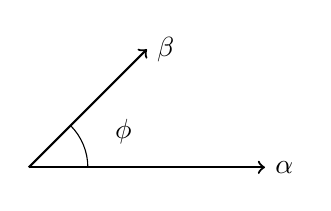
\begin{tikzpicture}[scale=1.5]
        \draw[->,thick] (0,0) -- (2,0) node[anchor=west] {\(\alpha\)};
        \draw[->,thick] (0,0) -- (1,1) node[anchor=west] {\(\beta\)};
        \draw (0.5,0) arc (0:45:0.5);
        \draw (0.8,0.3) node {\(\phi\)};
    \end{tikzpicture}
    \label{fig:rootangle}
\end{figure}

We have:
\begin{align}
    R_{\alpha,\beta} = \frac{2(\alpha,\beta)}{(\alpha,\alpha)} = 2\frac{|\beta|}{|\alpha|}\cos\phi\in\ZZ \\
    R_{\beta,\alpha} = \frac{2(\alpha,\beta)}{(\beta,\beta)} = 2\frac{|\alpha|}{|\beta|}\cos\phi\in\ZZ \\
\end{align}
Multiplying these together we obtain:
\begin{equation}
    4 \cos^2\phi \in \ZZ \implies \cos\phi = \pm\frac{\sqrt{n}}{2} \text{ where } n \in \{0,1,2,3,4\}
\end{equation}
This constraint has the following solutions:
\begin{equation}
    \phi = 
    \begin{cases}
        0 & (\alpha=\beta) \\
        \frac{\pi}{2} & ((\alpha,\beta) = 0) \\
        \pi & (\alpha = -\beta) \\
        \frac{\pi}{6},\frac{\pi}{4},\frac{\pi}{3} & ((\alpha,\beta) > 0) \\
        \frac{5\pi}{6},\frac{3\pi}{4},\frac{2\pi}{3} & ((\alpha,\beta) < 0)
    \end{cases}
\end{equation}

\subsection{Simple roots}
\begin{defn}
    Choose some hyperplane in \(\mathfrak{h}^*\). We can divide the root set into \emph{positive roots} in \(\Phi_+\) and \emph{negative roots} in \(\Phi_-\) by imposing that positive roots lie on one side of the hyperplane, and negative roots on the other.
    \begin{figure}[H]
        \centering
        \begin{tikzpicture}[thick]
            \draw[dashed] (-4,2) -- (4,-2) node[near start, above, sloped] {hyperplane};
            \draw[->] (0,0) -- (2,1) node[anchor=west] {\(\beta\)};
            \draw[->] (0,0) -- (-2,-1) node[anchor=east] {\(-\beta\)};
            \draw[->] (0,0) -- (-1,3) node[anchor=south] {\(\delta\)};
            \draw[->] (0,0) -- (1,-3) node[anchor=north] {\(-\delta\)};
            \draw[->] (0,0) -- (4,0) node[anchor=west] {\(\alpha\)};
            \draw[->] (0,0) -- (-4,0) node[anchor=east] {\(-\alpha\)};
        \end{tikzpicture}
        \label{fig:hyperplane}
    \end{figure}
\end{defn}
This is equivalent to dividing \(\Phi = \Phi_+ \cup \Phi_-\) such that, for all roots \(\alpha,\beta\):
\begin{enumerate}[label=(\roman*)]
    \item \(\alpha \in \Phi_+ \iff -\alpha \in \Phi_-\).
    \item \(\alpha,\beta \in \Phi_+, \alpha+\beta \in \Phi \implies \alpha+\beta \in \Phi_+\).
\end{enumerate}

\begin{defn}
    A \emph{simple root} is a positive root which cannot be written as the sum of two positive roots. The set of simple roots is denoted \(\Phi_S\).
\end{defn}

\begin{lemma}
    \begin{enumerate}[label=(\roman*)]
        \item \(\alpha,\beta \in \Phi_S \implies \alpha-\beta \not\in \Phi\).
            \begin{proof}
                Suppose \(\alpha-\beta \in \Phi\). Then we have two cases:
                \begin{itemize}
                    \item \(\alpha-\beta \in \Phi_+ \implies \alpha = (\alpha-\beta) + \beta \implies \alpha\) not simple.
                    \item \(\alpha-\beta \in \Phi_- \implies \beta-\alpha \in \Phi_+ \implies \beta = (\beta-\alpha)+\alpha \implies \beta\) not simple. \qedhere
                \end{itemize}
            \end{proof}
        \item \(\alpha,\beta \in \Phi_S \implies S_{\alpha,\beta}\), the \(\alpha\)-string through \(\beta\), has length \(l_{\alpha,\beta} = 1 - \frac{2(\alpha,\beta)}{(\alpha,\alpha)} \in \NN\).
            \begin{proof}
                Recall that we can write \(S_{\alpha,\beta} = \{\beta+n\alpha;\, n \in \ZZ, n_- \le n \le n_+\}\) with \(n_+\ge0,n_-\le0\), and \(n_++n_- = - \frac{2(\alpha,\beta)}{(\alpha,\alpha)} \in \ZZ\). Now, (i) implies that \(n_- = 0\). Hence, \(n_+ = - \frac{2(\alpha,\beta)}{(\alpha,\alpha)}\) and so \(l_{\alpha,\beta} = n_+-n_-+1 = 1 - \frac{2(\alpha,\beta)}{(\alpha,\alpha)} \in \NN\).
            \end{proof}
        \item \(\alpha,\beta \in \Phi_S, \alpha \ne \beta \implies (\alpha,\beta) \le 0\). \emph{(This is a corollary of \emph{(ii)}.)}
        \item Any positive root \(\beta\) can be written as a linear combination of simple roots with positive integer coefficients.
            \begin{proof}
                If \(\beta \in \Phi_S\), then we are done. If \(\beta \ne \Phi_S\) then we can write \(\beta = \beta_1 + \beta_2\) for some positive roots \(\beta_1,\beta_2\). Since the rank is finite, we can iterate on this until all of the \(\beta_i\) are simple roots, and then we are done.
            \end{proof}
        \item All roots \(\alpha \in \Phi\) can be written as \(\alpha = \sum_i d_i \alpha_{(i)}\) with \(d_i \in \ZZ, \alpha_{(i)} \in \Phi_S\), so the simple roots span \(\mathfrak{h}^*_\RR\). \emph{(This is a corollary of \emph{(iv)}.)}
        \item Simple roots are linearly independent.
            \begin{proof}
                Consider all vectors \(\lambda \in \mathfrak{h}^*_\RR\). By \emph{(v)} we can write \(\lambda = \sum_i c_i\alpha_{(i)}\) where \(c_i \in \RR, \alpha_{(i)} \in \Phi_S\). Restrict to the case where not all \(c_i = 0\). Let \(J_\pm = \{i \st c_i \gtrless 0\}\), and \(\lambda_\pm = \pm\sum_{i \in J_\pm}c_i\alpha_{(i)}\); we have \(\lambda = \lambda_+-\lambda_-\). Then 
                \begin{align}
                    (\lambda,\lambda) &= (\lambda_+,\lambda_+) + (\lambda_-,\lambda_-) - 2(\lambda_+,\lambda_-) \\
                    &> -2(\lambda_+,\lambda_-) \\
                    &= +2\sum_{i\in J_+}\sum_{j\in J_-} \underbrace{c_ic_j}_{< 0} \underbrace{(\alpha_{(i)},\alpha_{(j)})}_{\le 0 \text{ (by \emph{(iii)})}} \\
                    & \ge 0
                \end{align}
                Hence \((\lambda,\lambda) > 0\). So \((\lambda,\lambda) = 0\) if and only if \(c_i = 0 \Forall i\).
            \end{proof}
        \item There are exactly \(r=\operatorname{rank}[\mathfrak{g}]\) simple roots.
            \begin{proof}
                \emph{(v)} and \emph{(vi)} tell us that \(\Phi_S\) is a basis of \(\mathfrak{h}^*_\RR\). Hence \(|\Phi_S| = \dim\mathfrak{h}^*_\RR=r\).
            \end{proof}
    \end{enumerate}
\end{lemma}

From now on we will label simple roots as \(\alpha_{(i)}, i=1,\dots,r\).
\begin{defn}
    The \emph{Cartan matrix} of a Lie algebra is an \(r\times r\) matrix \(A\) with components given by:
    \begin{equation}
        A^{ij} = \frac{2(\alpha_{(i)},\alpha_{(j)})}{(\alpha_{(j)},\alpha_{(j)})} \in \ZZ
    \end{equation}
\end{defn}
Note that \(A\) is not generally symmetric.

We can choose \(\{h^i=h^{\alpha_{(i)}},e_\pm^i=e^{\pm\alpha_{(i)}}\}\) as a basis for the Lie algebra. Then the Lie algebra structure is as follows:
\begin{align}
    [h^i,e_\pm^i] &= \pm2e_\pm^i \\
    [h^i,e_\pm^j] &= \pm A^{ji} e^j_\pm \\
    [e_+^i, e_-^i] &= h^i
\end{align}
with all other brackets \(=0\).

\subsection{Classification}
The Cartan classification of finite-dimensional simple complex Lie algebras has two steps:
\begin{enumerate}
    \item Classify all possible Cartan matrices.
    \item Show that a Cartan matrix uniquely determines each Lie algebra.
\end{enumerate}

So first let us examine the constraints on the Cartan matrix:
\begin{enumerate}[label=(\alph*)]
    \item \(A^{ii} = 2 \Forall i\).
    \item Symmetry of the linear product gives \(A^{ij} = 0 \iff A^{ji} = 0\).
    \item \((\alpha,\beta) \le 0\) for \(\alpha \ne \beta \in \Phi_S \implies A^{ij} \in \ZZ^{\le 0}\) for all \(i \ne j\).
    \item Euclidean inner product implies \(\det A > 0\).
    \item \(\mathfrak{g}\) simple implies \(A\) is not reducible.
\end{enumerate}

\begin{eg}
    Consider \(r=2\). Then we have:
    \begin{equation}
        A = 
        \begin{pmatrix}
            2 & -m \\
            -n & 2
        \end{pmatrix}
    \end{equation}
    where \(m,n>0\) and \(\det A = 4-mn > 0\). So, up to exchange of \(m\) and \(n\), we have \((m,n) \in \{(1,1),(1,2),(1,3)\}\).
\end{eg}

It can be shown that \(A^{ij}A^{ji} \in \{0,1,2,3\}\) (no summation), and that simple complex Lie algebras can have roots of at most 2 distinct lengths.

To represent the structure of a Lie algebra, we use \emph{Dynkin diagrams}, which we construct in the following way:
\begin{itemize}
    \item Draw a node \tikz\draw (0,0) circle (0.1); for each simple root \(\alpha_{(i)}\).
    \item Join the nodes representing \(\alpha_{(i)}\) and \(\alpha_{(j)}\) with \(\max(|A^{ij}|,|A^{ji}|) \in \{0,1,2,3\}\) lines.
    \item If more than one line connects two nodes, draw an arrowhead pointing from the longer root to the shorter one.
\end{itemize}

\begin{eg}
    In rank 2, there are three possible Cartan matrices and associated Dynkin diagrams:
    \begin{align}
        \begin{pmatrix}
            2 & -1 \\
            -1 & 2
        \end{pmatrix} &\quad
        \begin{tikzpicture}
            \draw (0,0) -- (1,0);
            \draw[fill=ExampleColor!4] (0,0) circle (0.15);
            \draw[fill=ExampleColor!4] (1,0) circle (0.15);
        \end{tikzpicture} \\
        \begin{pmatrix}
            2 & -2 \\
            -1 & 2
        \end{pmatrix} &\quad
        \begin{tikzpicture}
            \draw (0,0.03) -- (1,0.03);
            \draw (0,-0.03) -- (1,-0.03);
            \begin{scope}[xshift=15,scale=0.15]
                \draw (-1,1) -- (1,0) -- (-1,-1);
            \end{scope}
            \draw[fill=ExampleColor!4] (0,0) circle (0.15);
            \draw[fill=ExampleColor!4] (1,0) circle (0.15);
        \end{tikzpicture} \\
        \begin{pmatrix}
            2 & -3 \\
            -1 & 2
        \end{pmatrix} &\quad
        \begin{tikzpicture}
            \draw (0,0.06) -- (1,0.06);
            \draw (0,0) -- (1,0);
            \draw (0,-0.06) -- (1,-0.06);
            \begin{scope}[xshift=15,scale=0.15]
                \draw (-1,1) -- (1,0) -- (-1,-1);
            \end{scope}
            \draw[fill=ExampleColor!4] (0,0) circle (0.15);
            \draw[fill=ExampleColor!4] (1,0) circle (0.15);
        \end{tikzpicture}
    \end{align}
\end{eg}

\begin{theorem}[The Cartan classification]
    All finite-dimensional complex simple Lie algebras must have Dynkin diagrams of one of the following forms:
    \begin{align}
        A_n :&\quad
        \raisebox{-.5\height}{
        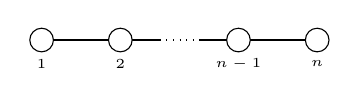
\begin{tikzpicture}
            \draw (0,0) -- (1.5,0);
            \draw[dotted] (1.5,0) -- (2,0);
            \draw (2,0) -- (3.5,0);
            \foreach \i in {1,...,2} {
                \draw[fill=white] (\i-1,0) circle (0.15);
                \draw (\i-1,-0.3) node[font=\tiny] {\(\i\)};
            }
            \draw[fill=white] (2.5,0) circle (0.15);
            \draw (2.5,-0.3) node[font=\tiny] {\(n-1\)};
            \draw[fill=white] (3.5,0) circle (0.15);
            \draw (3.5,-0.3) node[font=\tiny] {\(n\)};
        \end{tikzpicture}} \quad (\mathcal{L}_\CC(SU(n+1)))\\
        B_n :&\quad
        \raisebox{-.5\height}{
        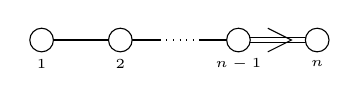
\begin{tikzpicture}
            \draw (0,0) -- (1.5,0);
            \draw[dotted] (1.5,0) -- (2,0);
            \draw (2,0) -- (2.5,0);
            \draw (2.5,0.03) -- (3.5,0.03);
            \draw (2.5,-0.03) -- (3.5,-0.03);
            \begin{scope}[xshift=86,scale=0.15]
                \draw (-1,1) -- (1,0) -- (-1,-1);
            \end{scope}
            \foreach \i in {1,...,2} {
                \draw[fill=white] (\i-1,0) circle (0.15);
                \draw (\i-1,-0.3) node[font=\tiny] {\(\i\)};
            }
            \draw[fill=white] (2.5,0) circle (0.15);
            \draw (2.5,-0.3) node[font=\tiny] {\(n-1\)};
            \draw[fill=white] (3.5,0) circle (0.15);
            \draw (3.5,-0.3) node[font=\tiny] {\(n\)};
        \end{tikzpicture}} \quad (\mathcal{L}_\CC(SO(2n+1)))\\
        C_n :&\quad
        \raisebox{-.5\height}{
        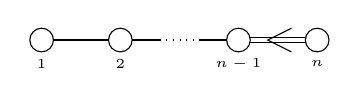
\begin{tikzpicture}
            \draw (0,0) -- (1.5,0);
            \draw[dotted] (1.5,0) -- (2,0);
            \draw (2,0) -- (2.5,0);
            \draw (2.5,0.03) -- (3.5,0.03);
            \draw (2.5,-0.03) -- (3.5,-0.03);
            \begin{scope}[xshift=86,scale=0.15]
                \draw (1,1) -- (-1,0) -- (1,-1);
            \end{scope}
            \foreach \i in {1,...,2} {
                \draw[fill=white] (\i-1,0) circle (0.15);
                \draw (\i-1,-0.3) node[font=\tiny] {\(\i\)};
            }
            \draw[fill=white] (2.5,0) circle (0.15);
            \draw (2.5,-0.3) node[font=\tiny] {\(n-1\)};
            \draw[fill=white] (3.5,0) circle (0.15);
            \draw (3.5,-0.3) node[font=\tiny] {\(n\)};
        \end{tikzpicture}} \quad (\mathcal{L}_\CC(SP(2n)))\\
        D_n :&\quad
        \raisebox{-.5\height}{
        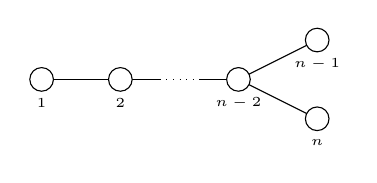
\begin{tikzpicture}
            \draw (0,0) -- (1.5,0);
            \draw[dotted] (1.5,0) -- (2,0);
            \draw (2,0) -- (2.5,0);
            \draw (2.5,0) -- (3.5,0.5);
            \draw (2.5,0) -- (3.5,-0.5);
            \foreach \i in {1,...,2} {
                \draw[fill=white] (\i-1,0) circle (0.15);
                \draw (\i-1,-0.3) node[font=\tiny] {\(\i\)};
            }
            \draw[fill=white] (2.5,0) circle (0.15);
            \draw (2.5,-0.3) node[font=\tiny] {\(n-2\)};
            \draw[fill=white] (3.5,0.5) circle (0.15);
            \draw (3.5,0.2) node[font=\tiny] {\(n-1\)};
            \draw[fill=white] (3.5,-0.5) circle (0.15);
            \draw (3.5,-0.8) node[font=\tiny] {\(n\)};
        \end{tikzpicture}} \quad (\mathcal{L}_\CC(SO(2n)))
    \end{align}
    or be one of five exceptional cases:
    \begin{align}
        E_6 :&\quad 
        \raisebox{-.5\height}{
        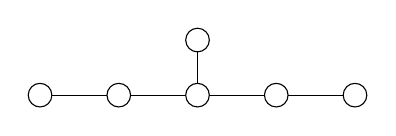
\begin{tikzpicture}
            \draw (0,0) -- (4,0);
            \draw (2,0) -- (2,0.7);
            \foreach \i in {1,...,5} {
                \draw[fill=white] (\i-1,0) circle (0.15);
            }
            \draw[fill=white] (2,0.7) circle (0.15);
        \end{tikzpicture}}\\
        E_7 :&\quad 
        \raisebox{-.5\height}{
        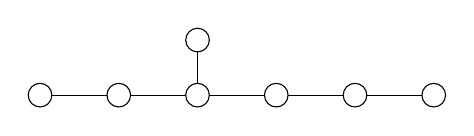
\begin{tikzpicture}
            \draw (0,0) -- (5,0);
            \draw (2,0) -- (2,0.7);
            \foreach \i in {1,...,6} {
                \draw[fill=white] (\i-1,0) circle (0.15);
            }
            \draw[fill=white] (2,0.7) circle (0.15);
        \end{tikzpicture}}\\
        E_8 :&\quad 
        \raisebox{-.5\height}{
        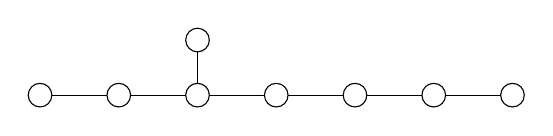
\begin{tikzpicture}
            \draw (0,0) -- (6,0);
            \draw (2,0) -- (2,0.7);
            \foreach \i in {1,...,7} {
                \draw[fill=white] (\i-1,0) circle (0.15);
            }
            \draw[fill=white] (2,0.7) circle (0.15);
        \end{tikzpicture}}\\
        F_4 :&\quad
        \raisebox{-.35\height}{
        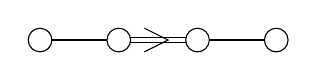
\begin{tikzpicture}
            \draw (0,0) -- (1,0);
            \draw (1,0.03) -- (2,0.03);
            \draw (1,-0.03) -- (2,-0.03);
            \draw (2,0) -- (3,0);
            \begin{scope}[xshift=42,scale=0.15]
                \draw (-1,1) -- (1,0) -- (-1,-1);
            \end{scope}
            \foreach \i in {1,...,4} {
                \draw[fill=white] (\i-1,0) circle (0.15);
            }
        \end{tikzpicture}} \\
        G_2 :&\quad
        \raisebox{-.2\height}{
        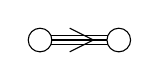
\begin{tikzpicture}
            \draw (0,0.06) -- (1,0.06);
            \draw (0,0) -- (1,0);
            \draw (0,-0.06) -- (1,-0.06);
            \begin{scope}[xshift=15,scale=0.15]
                \draw (-1,1) -- (1,0) -- (-1,-1);
            \end{scope}
            \draw[fill=white] (0,0) circle (0.15);
            \draw[fill=white] (1,0) circle (0.15);
        \end{tikzpicture}}
    \end{align}
\end{theorem}

\begin{eg}
    \(A_1=B_1=C_1\), and \(D_1\) isn't a thing. So there is only one possible finite-dimensional complex simple Lie algebra of rank 1. We can deduce:
    \begin{equation}
        \mathcal{L}_\CC(SU(2)) \simeq \mathcal{L}_\CC(SO(3)) \simeq \mathcal{L}_\CC(SP(2))
    \end{equation}
\end{eg}
\begin{eg}
    In rank 2, we recover the above Dynkin diagrams. The diagrams for \(B_2\) and \(C_2\) are identical, so we can say \(\mathcal{L}_\CC(SO(5)) \simeq \mathcal{L}_\CC(SP(4))\). Note that \(D_2\)'s diagram is the same as two \(A_1\)s, so we can say \(\mathcal{L}_\CC(SO(4)) \simeq \mathcal{L}_\CC(SU(2)) \oplus \mathcal{L}_\CC(SU(2))\).
\end{eg}

Now that we know which Dynkin diagrams are avaliable, how do we reconstruct a Lie algebra \(\mathfrak{g}\)? First we must determine the Cartan matrix \(A\), which can be easily read off from the diagram. \(A\) then determines the simple roots in \(\mathfrak{h}^*_\RR\) (up to one undetermined vector). From the simple roots we can then reconstruct all roots by forming root strings with length \(l_{ij}=1-A_{ji} \in \NN\).

\begin{eg}
    Consider the Dynkin diagram for \(A_2\). 
    \begin{figure}[H]
        \centering
        \begin{tikzpicture}
            \draw (0,0) -- (1,0);
            \draw[fill=ExampleColor!4] (0,0) circle (0.15);
            \draw[fill=ExampleColor!4] (1,0) circle (0.15);
        \end{tikzpicture}
    \end{figure}
    We can see that we must have Cartan matrix given by 
    \begin{equation}
        A = 
        \begin{pmatrix}
            2 & -1 \\
            -1 & 2
        \end{pmatrix}
    \end{equation}
    Call the simple roots \(\alpha\) and \(\beta\). We have:
    \begin{equation}
        \frac{2(\alpha,\beta)}{(\alpha,\alpha)} = \frac{2(\alpha,\beta)}{(\beta,\beta)} = -1\\
    \end{equation}
    \begin{equation}
        \implies \frac{2|\alpha|}{|\beta|}\cos\phi = \frac{2|\beta|}{|\alpha|}\cos\phi = -1
    \end{equation}
    \begin{equation}
        \implies |\beta|=|\alpha|,\; \phi = \frac{2\pi}{3}
    \end{equation}
    The length of the \(\alpha\)-string through \(\beta\) is \(l_{\alpha,\beta} =  1 - \frac{2(\alpha,\beta)}{(\alpha,\alpha)} = 2\), so \(\alpha+\beta\) is a root. No extra roots arise from the other strings. We also have negative roots \(-\alpha,-\beta,-\alpha-\beta\). So the full set of roots is \(\Phi=\{\alpha,\beta,-\alpha,-\beta,\alpha+\beta,-\alpha-\beta\}\):
    \begin{figure}[H]
        \centering
        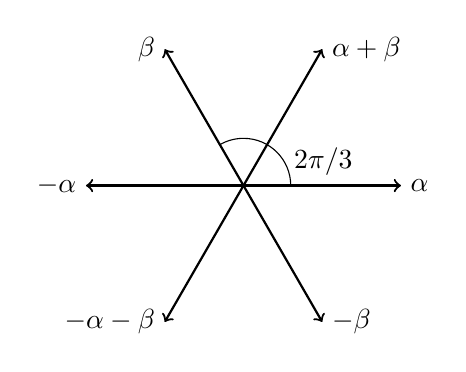
\begin{tikzpicture}
            \foreach \i in {0,...,5} {
                \draw[rotate={60*\i},thick,->] (0,0) -- (2,0);
            }
            \draw (2,0) node[anchor=west] {\(\alpha\)};
            \draw[rotate=60] (2,0) node[anchor=west] {\(\alpha+\beta\)};
            \draw[rotate=120] (2,0) node[anchor=east] {\(\beta\)};
            \draw[rotate=180] (2,0) node[anchor=east] {\(-\alpha\)};
            \draw[rotate=240] (2,0) node[anchor=east] {\(-\alpha-\beta\)};
            \draw[rotate=300] (2,0) node[anchor=west] {\(-\beta\)};
            \draw (0.6,0) arc (0:120:0.6) node[near start, anchor=west] {\(2\pi/3\)};
        \end{tikzpicture}
    \end{figure}
\end{eg}

\section{More representations}
\subsection{Representation theory of Lie algebras}

Suppose \(R\) is a representation of \(\mathfrak{g}\). \(R\) takes elements of the Cartan-Weyl basis to \(\operatorname{Mat}_N(\CC)\).
\begin{align}
    H^i &\mapsto R(H^i) \\
    E^\alpha &\mapsto R(E^\alpha)
\end{align}
Let's assume \(R(H^i)\) is diagonalisable. Since \([R(H^i),R(H^j)] = R([H^i,H^j]) = 0\), the \(R(H^i)\) are simultaneously diagonalisable. \(V=\CC^N\) is spanned by the eigenvectors of \(\{R(H^i)\}\). We can write \(V=\bigoplus_{\lambda\in S_R}V_\lambda\), where if \(v \in V_\lambda\) then \(R(H^i)v=\lambda^iv\), and \(\lambda^i \in \CC, i=1,\dots,r\). \(\lambda\) is called a \emph{weight} of \(R\); the set of weights \(S_R\) is called its \emph{weight set}. Weights in general can have non-trivial multiplicity \(m_\lambda= \dim V_\lambda \ge 1\).
\begin{eg}
    The roots are the weights for the adjoint representation.
\end{eg}
Consider the action of the representations of the step operators \(R(E^\alpha)\) on \(v \in V_\lambda\):
\begin{align}
    R(H^i)R(E^\alpha)v &= (R(E^\alpha)R(H^i) + [R(H^i),R(E^\alpha)])v \\
    &= \lambda^i R(E^\alpha)v + R([H^i,E^\alpha])v \\
    &= (\lambda^i + \alpha^i)R(E^\alpha)v
\end{align}
So \(R(E^{\alpha})v \in V_{\lambda+\alpha}\) if it is non-zero.

Recall that we have a set of \(sl(2)\) generators for each simple root \(\{h^i=h^{\alpha_{(i)}},\,e^i_\pm = e^{\pm\alpha_{(i)}}\}\), obeying:
\begin{align}
    [h^i,h^j] &= 0\\
    [h^i,e_\pm^j] &= \pm A^{ji}e^j_\pm \\
    [e^i_+,e^i_-] &= h^i
\end{align}
with \([e^i_\pm,e^j_\pm]\) generating new basis elements, and all other brackets \(=0\). We have:
\begin{equation}
    [e_+^i,e_+^j] = \operatorname{ad}_{e^i_+}
    \begin{cases}
        \propto e^{\alpha_{(j)}+\alpha_{(i)}} & \text{if } \alpha_{(j)}+\alpha_{(i)} \in \Phi \\
        = 0 & \text{otherwise}
    \end{cases}
\end{equation}
Since the \(\alpha_{(i)}\)-string through \(\alpha_{(j)}\) has length \(1-A_{ji}\), we can deduce the \emph{Serre relation}:
\begin{equation}
    ( \operatorname{ad}_{e_\pm^i} )^{1-A^{ji}}e_\pm^j = 0
\end{equation}
It can be shown that the Serre relation together with the set of bracket relations for \(sl(2)_{\alpha_{(i)}}\) uniquely determines \(\mathfrak{g}\); this is called \emph{Serre reconstruction}.

Considering the action of the \(sl(2)_\alpha\) generators on \(V\), we can see that \(V\) is a representation space to some representation \(R_\alpha\) of \(sl(2)_\alpha\) (in general \(R_\alpha\) is reducible). For all \(v \in V_\lambda\), we have:
\begin{align}
    R(h^\alpha)v &= \frac{2}{(\alpha,\alpha)}(\kappa^-1)_{ij}\alpha^iR(H^j)v \\
    &= \frac{2}{(\alpha,\alpha)}(\kappa^-1)_{ij}\alpha^i\lambda^j \\
    &= \frac{2(\alpha,\lambda)}{\alpha,\alpha} v
\end{align}
So \(\frac{2(\alpha,\lambda)}{(\alpha,\alpha)} \in \ZZ\) for all \(\lambda \in S_R, \alpha \in \Phi\).

\subsection{Root and weight lattices}
\begin{defn}
    The \emph{root lattice} \(\mathcal{L}[\mathfrak{g}]\) of a Lie algebra \(\mathfrak{g}\) with simple roots \(\alpha_{(i)}\) is defined by:
    \begin{equation}
        \mathcal{L}[\mathfrak{g}] = \operatorname{span}_\ZZ\{\alpha_{(i)}\}
    \end{equation}
\end{defn}
\begin{defn}
    The \emph{simple coroots} \(\check{\alpha}_{(i)}\) of a Lie algebra \(\mathfrak{g}\) with simple roots \(\alpha_{(i)}\) are given by:
    \begin{equation}
        \check{\alpha}_{(i)} = \frac{2}{(\alpha_{(i)},\alpha_{(i)})}\alpha_{(i)}
    \end{equation}
\end{defn}
\begin{defn}
    The \emph{coroot lattice} \(\check{\mathcal{L}}[\mathfrak{g}]\) of a Lie algebra \(\mathfrak{g}\) with simple coroots \(\check{\alpha}_{(i)}\) is defined as:
    \begin{equation}
        \check{\mathcal{L}}[\mathfrak{g}] = \operatorname{span}_\ZZ \{\check{\alpha}_{(i)}\}
    \end{equation}
\end{defn}
\begin{defn}
    The \emph{weight lattice} \(\mathcal{L}_W[\mathfrak{g}]\) of a Lie algebra \(\mathfrak{g}\) is the dual lattice of its coroot lattice:
    \begin{equation}
        \mathcal{L}_W[\mathfrak{g}] = \check{\mathcal{L}}^*[\mathfrak{g}] = \{\lambda \in \mathfrak{h}^*_\RR \st (\lambda,\mu) \in \ZZ \Forall \mu \in \check{\mathcal{L}}[\mathfrak{g}]\}
    \end{equation}
\end{defn}
In particular:
\begin{equation}
    \lambda \in \mathcal{L}_W[\mathfrak{g}] \iff (\lambda,\check{\alpha}_{(i)}) = \frac{2(\alpha_{(i)},\lambda)}{(\alpha_{(i)},\alpha_{(i)})} \in \ZZ
\end{equation}
So the weights of any representation \(R\) of \(\mathfrak{g}\) all lie in \(\mathcal{L}_W[\mathfrak{g}]\). The simple coroots are a basis for the coroot lattice, so we have a dual basis for the weight lattice \(\{\omega_{(i)}\}\) where:
\begin{equation}
    (\check{\alpha}_{(i)},\omega_{(j)}) = \frac{2(\alpha_{(i)},\omega_{(j)})}{(\alpha_{(i)},\alpha_{(i)})} = \delta_{ij} \tag{\(*\)}
    \label{fundamentalweights}
\end{equation}
The \(\omega_{(i)}\) are called \emph{fundamental weights} of \(\mathfrak{g}\). Since the simple roots span \(\mathfrak{h}^*_\RR\), we can write \(\omega_{(i)} = \sum_{j=1}^r B_{ij} \alpha_{(j)}\) for some real matrix \(B\). With \eqref{fundamentalweights} this yields:
\begin{equation}
    \sum_{k=1}^r\frac{2(\alpha_{(i)},\alpha_{(k)})}{(\alpha_{(i)},\alpha_{(i)})} B_{jk} = A^{ki}B_{jk} = \delta^i_j
\end{equation}
In other words, \(B\) is the inverse of \(A\), so we can write:
\begin{equation}
    \alpha_{(i)} = \sum_{j=1}^rA^{ij}\omega_{(j)}
\end{equation}

\begin{eg}
    Consider \(\mathfrak{g}=A_2\). Then we have shown:
    \begin{equation}
        A = 
        \begin{pmatrix}
            2 & -1 \\
            -1 & 2
        \end{pmatrix}
    \end{equation}
    so:
    \begin{align}
        \alpha = \alpha_{(1)} &= 2 \omega_{(1)} - \omega_{(2)} \\
        \beta = \alpha_{(2)} &= - \omega_{(1)} + 2 \omega_{(2)}
    \end{align}
    Inverting these, we find:
    \begin{align}
        \omega_{(1)} &= \frac{1}{3}(2\alpha+\beta) \\
        \omega_{(2)} &= \frac{1}{3}(\alpha+2\beta)
    \end{align}
    \begin{figure}[H]
        \centering
        \begin{tikzpicture}[thick]
            \draw[->,dashed] (0,0) -- (4,0) node[anchor=west] {\(\alpha\)};
            \draw[->,dashed,rotate=120] (0,0) -- (4,0) node[anchor=south] {\(\beta\)};
            \draw[->] (0,0) -- (0,{4/sqrt(3)}) node[anchor=south] {\(\omega_{(2)}\)};
            \draw[->] (0,0) -- (2,{2/sqrt(3)}) node[anchor=west] {\(\omega_{(1)}\)};
            \fill (0,0) circle (0.07);
        \end{tikzpicture}
    \end{figure}
\end{eg}

Any weight \(\lambda \in S_R \subset \mathcal{L}_W[\mathfrak{g}]\) can be written as a linear combination of the fundamental weights:
\begin{equation}
    \lambda = \sum_{i=1}^r \lambda^i\omega_{(i)}
\end{equation}
\(\lambda^i \in \ZZ\) are known as the \emph{Dynkin labels} of \(\lambda\).

Every finite dimensional representation \(R\) of \(\mathfrak{g}\) has a highest weight, i.e. a \(\Lambda \in S_R\) such that \(R(E^\alpha)v = 0\) for all \(\alpha \in \Phi_+\) and \(v \in V_\Lambda\). If the highest weight is unique and non-degenerate, then \(R_\Lambda\) is a finite dimensional irreducible representation. The rest of the states in the irrep can be found by acting with lowering generators \(R(E^{-\alpha}), \alpha \in \Phi_+\) on \(V_\Lambda\):
\begin{equation}
    v_\lambda = R(E^{-\alpha_1})R(E^{-\alpha_2}) \dots R(E^{-\alpha_l}) v_\Lambda
\end{equation}
Every weight of the representation, which we will call \(R_\Lambda\), can be written as:
\begin{equation}
    \lambda = \Lambda-\mu \text{ where } \mu = \sum_{i=1}^r\mu^i\alpha_{(i)}, \mu^i \in \ZZ, \mu^i \ge 0
\end{equation}
The highest weight is also sometimes called the \emph{dominant weight}.

The following is a useful result:
\begin{lemma}
    For any finite dimensional representation of \(\mathfrak{g}\), if \(\lambda = \sum_{i=1}^r \lambda^i \omega_{(i)} \in S_R\) then \(\lambda-m_{(i)}\alpha_{(i)} \in S_R\) where \(m_{(i)} \in \ZZ, 0 \le m_{(i)} \le \lambda^i\).
\end{lemma}

\begin{eg}
    Consider \(\mathfrak{g}=A_2\), the fundamental representation has highest weight Dynkin labels \((1,0) = (\Lambda^1,\Lambda^2)\). This implies \(\Lambda = \omega_{(1)} \in S_f\), which then by the proposition implies \(\Lambda-\alpha_{(1)} = -\omega_{(1)}+\omega_{(2)} \in S_f\). Applying the proposition again, we have \(-\omega_{(1)}+\omega_{(2)} -\alpha{(2)} = -\omega_{(2)} \in S_f\). There are no more weights, so we have:
    \begin{equation}
        S_f = \{\omega_{(1)},-\omega_{(1)}+\omega_{(2)},-\omega_{(2)}\}
    \end{equation}
\end{eg}

\begin{eg}
    Consider general irreps of \(A_2\). For each dominant integral weight \(\Lambda\), we can write \(\Lambda = \Lambda^1\omega_{(1)}+\Lambda^2\omega_{(2)}\), with \(0 \le \Lambda^1,\Lambda^2  \in \ZZ\), and we get an irrep \(R_{(\Lambda^1,\Lambda^2)}\) of \(A_2\). It can be shown that:
    \begin{itemize}
        \item \(\dim R_{(\Lambda^1,\Lambda^2)} = \frac{1}{2}(\Lambda^1+1)(\Lambda^2+1)(\Lambda^1+\Lambda^2+2)\).
        \item If \(\Lambda^1 \ne \Lambda^2\) then we have \(R_{(\Lambda^1,\Lambda^2)} = \bar{R}_{(\Lambda^2,\Lambda^1)}\) and \(\lambda \in S_{(\Lambda^1,\Lambda^2)} \implies -\lambda \in S_{(\Lambda^2,\Lambda^1)}\).
    \end{itemize}
\end{eg}

\section{Symmetries in Quantum Mechanics}
Consider a generic quantum mechanical system with energy levels \(E_0 < E_1 < E_2 < \dots\) for a Hamiltonian \(\hat{H}\). The states of the system are elements of a Hilbert space:
\begin{equation}
    \mathcal{H} = \bigoplus_{n\ge0}\mathcal{H}_n \text{ where } \hat{H}\ket{\psi} = E_n\ket{\psi} \Forall \ket{\psi}\in\mathcal{H}_n
\end{equation}

\begin{defn}
    A \emph{symmetry transformation} of a system is a transformation \(\ket{\psi} \mapsto \ket{\psi'} = \hat{U}\ket{\psi}\), where \(\hat{U}:\mathcal{H}\rightarrow\mathcal{H}\) is a unitary operator such that \(\hat{U}\hat{H}\herm{\hat{U}} = \hat{H}\).
\end{defn}

Under a symmetry transformation, the inner product is preserved, and the energy is invariant.

\begin{defn}
    A \emph{conserved quantity} is an observable \(\hat{I}=\herm{\hat{I}}\) such that \([\hat{I},\hat{H}] = 0\).
\end{defn}

If \(\hat{I}\) is conserved, then \(\hat{U} = \exp(is\hat{I}), s \in \RR\) is a symmetry transformation.

Suppose we have a maximal set of linearly independent conserved quantities \(\{\hat{I}^a \st [\hat{I}^a,\hat{H}] = 0, a = 1,\dots,d\}\). Then \(\mathfrak{g}_\RR=\operatorname{span}_\RR\{i\hat{I}^a;\,a=1,\dots,d\}\) is a real Lie algebra with bracket equal to the operator commutator.

Consider all symmetry transformations of the form \(\hat{U} = \exp(\hat{X})\) where \(\hat{X}\in\mathfrak{g}_\RR\). These form a Lie group \(G\), and moreover \(G\) is compact (since \(G\) is a subgroup of some product of unitary groups). As \([\hat{X},\hat{H}] = 0 \Forall \hat{X}\in\mathfrak{g}_\RR\), the \(\mathcal{H}_n\) are invariant under the action of \(G\) or \(\mathfrak{g}_\RR\).

Each \(\mathcal{H}_n\) carries a representation \(D_n\) of \(G\), \(d_n\) of \(\mathfrak{g}_\RR\) such that \(D_n(\hat{U})=\exp(d_n(\hat{X})) \in \operatorname{Mat}_{N_n}(\CC)\) where \(N_n = \dim\mathcal{H}_n\). This representation must be \emph{unitary}, i.e.:
\begin{equation}
    D_n^{-1}(\hat{U}) = D_n(\hat{U}) \text{ or equivalently }  \herm{d_n(\hat{X})} = -d_n(\hat{X})
\end{equation}
Note that all finite dimensional representations of a compact \(G\) are automatically unitary.

\subsection{Hadronic physics}
Hadronic physics is the study of the hadrons: mesons (which are bosons) and baryons (which are fermions). The following isn't the most modern approach, but it is one of the first and simplest examples of the application of Lie theory to particle physics. We will refer to \emph{isospin} \(I\) and \emph{hypercharge} \(Y\). These are quantum numbers associated with the strong interaction; it is not necessary to know their details. The first few hadrons to be known about are listed below.

\begin{table}[H]
    \centering
    \subfloat[Mesons.]{
        \begin{tabular}{cccc} \toprule
            & \(Q\) & \(M\) & \(I\) \\ \midrule
            \(\pi^+\) & \(+1\) & \SI{139}{\mega\eV} & \(+1\) \\
            \(\pi^0\) & \(0\) & \SI{135}{\mega\eV} & \(0\) \\
            \(\pi^-\) & \(-1\) & \SI{139}{\mega\eV} & \(+1\) \\ \bottomrule
        \end{tabular}
    }
    \subfloat[Baryons.]{
        \begin{tabular}{cccc} \toprule
            & \(Q\) & \(M\) & \(I\) \\ \midrule
            \(p\) & \(+1\) & \SI{938}{\mega\eV} & \(+\frac{1}{2}\) \\
            \(n\) & \(0\) & \SI{940}{\mega\eV} & \(-\frac{1}{2}\) \\ \bottomrule
        \end{tabular}
    }
    \caption{The first few hadrons discovered.}
\end{table}

It was observed that isospin obeys an approximate \(SU(2)\) symmetry, with Cartan element \(H = 2I\). The proton and the neutron sit in the \(R_1\) representation, while the \(\pi\) mesons sit in the \(R_2\) representation:
\begin{align}
    \begin{pmatrix}
        \ket{p} \\ \ket{n}
    \end{pmatrix}
    &\sim R_1
    &
    \begin{pmatrix}
        \ket{\pi^+} \\ \ket{\pi^0} \\ \ket{\pi^-}
    \end{pmatrix}
    &\sim R_2
\end{align}

Soon many more mesons and baryons were discovered, along with the new conserved quantum number hypercharge and many unexplained approximate degeneracies. We can plot the 8 lightest mesons in the \(I\)-\(Y\) plane:
\begin{figure}[H]
    \centering
    \begin{tikzpicture}[scale=0.8]
        \draw[->,thick] (-4,0) -- (4,0) node[anchor=west] {\(I\)};
        \draw[->,thick] (0,-4) -- (0,4) node[anchor=south] {\(Y\)};
        \fill (0.2,-0.2) circle (0.1) node[anchor=north west] {\(\pi^0\)};
        \fill (-0.2,0.2) circle (0.1) node[anchor=south east] {\(\eta\)};
        \fill (3,0) circle (0.1) node[anchor=north] {\(\pi^+\)};
        \fill (-3,0) circle (0.1) node[anchor=north] {\(\pi^-\)};
        \fill ({3*cos(60)},{3*sin(60)}) circle (0.1) node[anchor=west] {\(K^+\)};
        \fill ({-3*cos(60)},{3*sin(60)}) circle (0.1) node[anchor=east] {\(K^0\)};
        \fill ({-3*cos(60)},{-3*sin(60)}) circle (0.1) node[anchor=east] {\(K^-\)};
        \fill ({3*cos(60)},{-3*sin(60)}) circle (0.1) node[anchor=west] {\(\bar{K}^0\)};
    \end{tikzpicture}
\end{figure}

The 8 lightest baryons form a similar shape:
\begin{figure}[H]
    \centering
    \begin{tikzpicture}[scale=0.8]
        \draw[->,thick] (-4,0) -- (4,0) node[anchor=west] {\(I\)};
        \draw[->,thick] (0,-4) -- (0,4) node[anchor=south] {\(Y\)};
        \fill (0.2,-0.2) circle (0.1) node[anchor=north west] {\(\Lambda\)};
        \fill (-0.2,0.2) circle (0.1) node[anchor=south east] {\(\varepsilon^0\)};
        \fill (3,0) circle (0.1) node[anchor=north] {\(\varepsilon^+\)};
        \fill (-3,0) circle (0.1) node[anchor=north] {\(\varepsilon^-\)};
        \fill ({3*cos(60)},{3*sin(60)}) circle (0.1) node[anchor=west] {\(p\)};
        \fill ({-3*cos(60)},{3*sin(60)}) circle (0.1) node[anchor=east] {\(n\)};
        \fill ({-3*cos(60)},{-3*sin(60)}) circle (0.1) node[anchor=east] {\(\Xi^-\)};
        \fill ({3*cos(60)},{-3*sin(60)}) circle (0.1) node[anchor=west] {\(\Xi^0\)};
    \end{tikzpicture}
\end{figure}

Consider now the Lie algebra \(\mathfrak{g}_\RR=\mathcal{L}(SU(3))\), and in particular its representation \(\underline{8} = R_{(1,1)}\). If we choose the following Cartan generators:
\begin{align}
    H^1 &=
    \begin{pmatrix}
        1 & 0 & 0 \\
        0 & -1 & 0 \\
        0 & 0 & 0
    \end{pmatrix}
    &
    H^2 &=
    \begin{pmatrix}
        0 & 0 & 0 \\
        0 & 1 & 0 \\
        0 & 0 & -1
    \end{pmatrix}
\end{align}
and set \(I = \frac{1}{2}H^1, Y= \frac{1}{3}(H^1+2H^2)\), then it is easy to calculate that the weights of \(R_{(1,1)}\) match the quantum numbers plotted above. If we do a similar investigation for the other known mesons and baryons, we find:
\begin{align}
    \text{Mesons live in: }& \underline{1}=R_{(0,0)} \text{ and } \underline{8}=R_{(1,1)} \text{,}\\
    \text{Baryons live in: }& \underline{8}=R_{(1,1)} \text{, } \underline{10}=R_{(3,0)} \text{ and } \underline{\bar{10}}=R_{(0,3)}
\end{align}
The immediate question to ask is: why only \(\underline{1},\underline{8}\) and \(\underline{10}\), and why do the mesons and baryons only live in their corresponding representations? There are more representations of \(SU(3)\), e.g. \(\underline{3},\underline{\bar{3}}, \underline{6}, \underline{\bar{6}}, \dots\)

The answer came from Gell-Mann, who proposed that all hadrons are composed of smaller more fundamental fermions called \emph{quarks}. Quarks live in \(\underline{3} = R_{(1,0)}\), and antiquarks live in \(\underline{\bar{3}} = R_{(0,1)}\). The key insight is to say that mesons are combinations of a quark and an antiquark, and that baryons are combinations of three quarks (or three antiquarks). 

Consider a meson in this regime. It has state given by \(\ket{\psi_1}\otimes\ket{\psi_2} \in \mathcal{H}_{(1)}\otimes \mathcal{H}_{(2)}\), where \(\ket{\psi_1},\ket{\psi_2}\) are the states of the quark and antiquark respectively. Suppose we have a conserved quantity \(\hat{I}_1\) on \(\mathcal{H}_{(1)}\) and \(\hat{I}_2\) on \(\mathcal{H}_{(2)}\). The operator corresponding to their sum for the entire meson is given by:
\begin{equation}
    I = \hat{I}_1 \otimes \identity_{(2)} + \identity_{(1)} \otimes \hat{I}_2
\end{equation}
We see that this is like the elements of the tensor product of two representation. Thus we can deduce that mesons (\(q\bar{q}\)) live in \(\underline{3}\otimes\underline{\bar{3}} = \underline{1} \oplus \underline{8}\). Similarly we have that baryons (\(qqq\)) live in \(\underline{3}\otimes\underline{3}\otimes\underline{3} = \underline{1}\oplus\underline{8}\oplus\underline{8}\oplus\underline{10}\). So we see exactly why the baryons and mesons have their representations.

In order to see exactly why we only have \(q\bar{q}\) and \(qqq\), it is necessary to study gauge QCD.

\subsection{Gauge Theory}

\begin{defn}
    A \emph{gauge symmetry} is a redundancy in the description of a system.
\end{defn}

\begin{eg}
    In classical electromagnetism, we define the non-observable scalar potential \(\Phi(\vb{x},t)\) and vector potential \(\vb{A}(\vb{x},t)\). What we then observe are the electric field \(\vb{E}=-\grad\Phi+\pdv{\vb{A}}{t}\) and magnetic field \(\vb{V} = \curl{\vb{A}}\). \(\vb{E}\) and \(\vb{B}\) are invariant under a gauge transformation given by:
    \begin{align}
        \Phi &\rightarrow \Phi + \pdv{\alpha}{t} \\
        \vb{A} &\rightarrow \vb{A} + \grad\alpha
    \end{align}
    where \(\alpha = \alpha(\vb{x},t)\) is some time-varying field. In a relativistic treatment we have a 4-vector potential \(a_\mu\) given by:
    \begin{equation}
        a_\mu = 
        \begin{cases}
            \Phi & \text{if } \mu = 0 \\
            A_i & \text{if } \mu = i = 1,2,3
        \end{cases}
    \end{equation}
    and gauge transformations \(a_\mu \rightarrow a_\mu + \partial_\mu\alpha\). The electric and magnetic fields live in the field-strength tensor \(f_{\mu\nu}\):
    \begin{align}
        f_{\mu\nu} &= \partial_\mu a_\nu - \partial_\nu a_\mu
        &
        E_i = f_{0i}, \, B_i = \frac{1}{2}\epsilon_{ijk}f_{jk}
    \end{align}
    We have a Lagrangian given by:
    \begin{equation}
        \mathcal{L}_\text{EM} = -\frac{1}{4g^2}f_{\mu\nu}f^{\mu\nu}
    \end{equation}
    where we use a Minkowski metric with signature \(+\)\(-\)\(-\)\(-\).

    Quantisation leads to a spin 1, massles, free particle that we call the \emph{photon}. For later convenience, we will define \(A_\mu = -ia_\mu\) and \(F_{\mu\nu} = -if_{\mu\nu}\).
\end{eg}

Consider a complex scalar field \(\phi:\RR^{3,1}\rightarrow\CC\) with Lagrangian given by:
\begin{equation}
    \mathcal{L}_\phi = \partial_\mu\phi^*\partial^\mu\phi - \underbrace{W(\phi^*\phi)}_\text{interactions}
\end{equation}
This Lagrangian is invariant under a global \(U(1)\) symmetry:
\begin{equation}
    \phi \rightarrow g \phi,\, \phi^* \rightarrow g^{-1}\phi^* \text{ where } g = \exp(i\delta) \in U(1),\, \delta \in [0,2\pi)
\end{equation}

Consider infinitesimal such transformations, i.e. those given by \(g=\exp(\epsilon X)\) where \(\epsilon \ll 1\) and \(X \in i\RR = \mathcal{L}(U(1))\). We have that \(g\approx1+\epsilon X\) so these transformations are: 
\begin{equation}
    \phi \rightarrow \phi + \delta_X\phi \text{ where } \delta_X\phi=\epsilon X\phi
\end{equation}
In general we will write \(\delta_Xx\) for the difference in a quantity \(x\) after the transformation. Working to first order in \(\epsilon\), we have \(\delta_X(\phi\phi^*) = 0\) and \(\delta_X\mathcal{L} = 0\) for all \(X \in i\RR\).

Now generalise \(X\) to depend on spacetime. We have \(\delta_X(\partial_\mu\phi) = \partial_\mu(\delta_X\phi) = \partial_\mu(\epsilon X\phi) = \epsilon \partial_\mu X \phi + \epsilon X \partial_\mu\phi\). Now \(\mathcal{L}_\phi\) is no longer invariant in general. In order to restore gauge-invariance, we replace all partial derivatives in the Lagrangian with a \emph{covariant derivative} \(D_\mu\), defined in the following way:
\begin{equation}
    D_\mu = \partial_\mu + A_\mu \text{ where } A_\mu : \RR^{3,1} \rightarrow \mathcal{L}(U(1)) = i\RR
\end{equation}
\(A_\mu\) is known as a \emph{\(U(1)\) gauge field} and must transform as \(\delta_XA_\mu = -\epsilon\partial_\mu X\). Then we have:
\begin{align}
    \delta_X(D_\mu\phi) &= \delta_X(\partial_\mu\phi + A_\mu\phi) \\
    &= \partial_\mu(\delta_X\phi) + (\delta_XA_\mu)\phi + A_\mu(\delta_X\phi) \\
    &= \partial_\mu(\epsilon X\phi) + A_\mu\epsilon X\phi - \epsilon\partial_\mu X\phi \\
    &= \epsilon \partial_\mu X\phi + \epsilon X\partial_\mu \phi + A_\mu\epsilon X\phi - \epsilon\partial_\mu X\phi \\
    &= \epsilon X D_\mu \phi
\end{align}
Thus, to first order, we have that \((D_\mu\phi)^*(D^\mu\phi)\) is gauge invariant. The most general gauge invariant Lagrangian we can have is:
\begin{equation}
    \mathcal{L} = \frac{1}{4g^2}F_{\mu\nu}F^{\mu\nu} + (D_\mu\phi)^*(D^\mu\phi) - W(\phi^*\phi)
\end{equation}
where \(F_{\mu\nu} = \partial_\mu A_\nu - \partial_\nu A_\mu\). It can be shown that if we want our theory to be renormalisable, we must further have \(W(Y) = \alpha Y + \beta Y^2\).

Now we will generalise this to any Lie group \(G\). Choose a representation \(D\) of \(G\) of dimension \(N\) with representation space \(V\simeq\CC^N\). We use the standard inner product \((u,v) = \herm{u}v\). Suppose we have a \(V\)-valued scalar field \(\phi:\RR^{3,1} \rightarrow V\), with the following Lagrangian:
\begin{equation}
    \mathcal{L}_\phi = (\partial_\mu\phi,\partial^\mu\phi) - W[(\phi,\phi)]
\end{equation}
If \(D\) is unitary (so \(\herm{D(g)} = D(g) = \identity\)), then \(\mathcal{L}_\phi\) is invariant under \(\phi \rightarrow D(g)\phi\) for all \(g \in G\). Near the identity, write \(g = \exp(\epsilon X)\) where \(\epsilon \ll 1\) and \(X \in \mathcal{L}(G)\). Then we have \(D(g) = \exp(\epsilon R(X))\) where \(R:\mathcal{L}(G)\rightarrow \operatorname{Mat}_N(\CC)\) defines a unitary representation of \(\mathcal{L}(G)\) (so \(R(X) = -\herm{R(X)}\)). For \(\epsilon \ll 1\), we have \(D(g) \approx \identity + \epsilon R(X)\). Under an infinitesimal transformation:
\begin{equation}
    \phi \rightarrow \phi + \delta_X\phi,\;\delta_X\phi = \epsilon R(X)\phi
\end{equation}
Now let's do what we did before and ``gauge'' the symmetry i.e. we let \(X\) be a \(\mathcal{L}(G)\) valued function of spacetime. Define the \emph{covariant derivative} by:
\begin{equation}
    D_\mu(\phi) = \partial_\mu\phi + R(A_\mu)\phi \text{ where } A_\mu:\RR^{3,1} \rightarrow \mathcal{L}(G)
\end{equation}
\(A_\mu\) is the gauge field for \(G\), and must transform as:
\begin{equation}
    \delta_XA_\mu = -\epsilon \partial_\mu X + \epsilon [X,A_\mu] \in \mathcal{L}(G)
\end{equation}
To see why, consider the action of the transformation on \(D_\mu \phi\):
\begin{align}
    \delta_X(D_\mu\phi) &= \delta_X(\partial_\mu\phi + R(A_\mu)\phi) \\
    &= \partial_\mu (\delta_X\phi) + R(A_\mu)\delta_X\phi + R(\delta_XA_\mu)\phi \\
    &= \partial_\mu (\epsilon R(X)\phi) + \epsilon R(A_\mu)R(X)\phi - \epsilon R(\partial_\mu X) + \epsilon R([X,A_\mu]) \\
    &= \epsilon(\partial_\mu R(X)) \phi + \epsilon R(X) \partial_\mu\phi + \epsilon R(X)R(A_\mu)\phi \\
    &\quad + \epsilon[R(A_\mu),R(X)]\phi - \epsilon R(\partial_\mu X)\phi + \epsilon[R(X),R(A_\mu)] \phi \\
    &= \epsilon R(X)D_\mu\phi
\end{align}
Thus:
\begin{equation}
    \delta_X[(D_\mu\phi,D^\mu\phi)] = \epsilon (R(X)D_\mu\phi,D^\mu\phi) + \epsilon (D_\mu\phi,R(X),D^\mu\phi) = 0
\end{equation}
since \(\herm{R(X)} = -R(X)\). Hence the Lagrangian is conserved.

Define the field-strength tensor as:
\begin{equation}
    F_{\mu\nu} = \partial_\mu A_\nu - \partial_\nu A_\mu + [A_\mu,A_\nu]
\end{equation}
Under a gauge transformation, we have:
\begin{align}
    \delta_X(F_{\mu\nu}) &= \partial_\mu(\delta_XA_\nu) - \partial_\nu(\delta_XA_\mu) + [\delta_XA_\mu,A_\nu] + [A_\mu,\delta_XA_\nu] \\
    &= -\epsilon\partial_\mu\partial_\nu X + \epsilon\partial_\mu([X,A_\nu]) + \epsilon \partial_\nu\partial_\mu X - \epsilon \partial_\nu([X,A_\mu]) \\
    &\quad -\epsilon[\partial_\mu X,A_\nu] - \epsilon[A_\mu, \partial_\nu X] + \epsilon [[X,A_\mu],A_\nu] + \epsilon [A_\mu,[X,A_\nu]] \\
    &= \epsilon[X,\partial_\mu A_\nu] - \epsilon[X,\partial_\nu A_\mu] - \epsilon([A_\nu,[X,A_\mu]] + [A_\mu,[A_\nu,X]]) \\
    &= \epsilon[X,\partial_\mu A_\nu - \partial_\nu A_\mu] + \epsilon[X,[A_\mu,A_\nu]] \\
    &= \epsilon[X,F_{\mu\nu}]
\end{align}
So for a gauge invariant Lagrangian that includes \(F_{\mu\nu}\), we can use the Killing form:
\begin{align}
    \mathcal{L}_A &= \frac{1}{g^2}\kappa(F_{\mu\nu},F^{\mu\nu}) \\
    \implies \delta_X\mathcal{L}_A &= \frac{1}{g^2}[\kappa(\delta_XF_{\mu\nu},F^{\mu\nu}) + \kappa(F_{\mu\nu},\delta_X)] \\
    &= \frac{\epsilon}{g^2}[\kappa([X,F_{\mu\nu}],F^{\mu\nu}) + \kappa(F_{\mu\nu},[X,F^{\mu\nu}])] \\
    &= 0
\end{align}
This provides a sensible kinetic term if \(\mathcal{L}(G)\) is of compact type. Note that \(\mathcal{L}_A\) contains both kinetic terms and interaction terms; if we take \(A \rightarrow gA\) then we have:

\begin{align}
    \mathcal{L}_A \sim && \partial A \partial A &&
    \raisebox{-.5\height}{\begin{tikzpicture}
        \exvertex{a}{0,0};
        \exvertex{b}{2,0};
        \gluon{a}{b};
    \end{tikzpicture}}
    &&
    \text{kinetic term}
    \\
    &&+ g[A,A]\partial A&&
    \raisebox{-.5\height}{\begin{tikzpicture}
        \exvertex{a}{-1,0};
        \exvertex{b}{{1*cos(60)},{1*sin(60)}};
        \exvertex{c}{{1*cos(60)},{-1*sin(60)}};
        \invertex{o}{0,0};
        \gluon{a}{o};
        \gluon{b}{o};
        \gluon{c}{o};
    \end{tikzpicture}}
    &&
    \text{3-vertex}
    \\
    &&+ g^2[A,A]^2&&
    \raisebox{-.5\height}{\begin{tikzpicture}
        \exvertex{a}{-1,0};
        \exvertex{b}{0,1};
        \exvertex{c}{1,0};
        \exvertex{d}{0,-1};
        \invertex{o}{0,0};
        \gluon{a}{o};
        \gluon{b}{o};
        \gluon{c}{o};
        \gluon{d}{o};
    \end{tikzpicture}}
    &&
    \text{4-vertex}
\end{align}

This is \emph{Yang-Mills} theory.

There is a large family of consistent gauge theories provided by the Cartan classification. We specify the following:
\begin{itemize}
    \item The gauge group is specified by the selection of a complex simple Lie algebra \(\mathfrak{g}_\CC\). This has a real form of compact type \(\mathfrak{g}_\RR\) that is equal to \(\mathcal{L}(G)\) for a compact Lie group \(G\).
    \item The matter content is specified by choosing a unitary representation of \(\mathfrak{g}_\RR\) for matter to live in. Then the matter field is \(\phi_\Lambda:\RR^{3,1} \rightarrow V_\Lambda\), where \(V_\Lambda\) is the representation space, and the subscript \(\Lambda\) specifies the dominant integral weights of the representation: \(\Lambda \in S = \{\text{dominant integral weights}\}\).
\end{itemize}

Then the most general possible Lagrangian for our theory is:
\begin{equation}
    \mathcal{L}_\Lambda = \frac{1}{g^2}\kappa(F_{\mu\nu},F^{\mu\nu}) + \sum_{\Lambda\in S} (D_\mu \phi_\Lambda,D^\mu \phi_\Lambda) - W\left( \{(\phi_\Lambda,\phi_\Lambda);\;\Lambda \in S \} \right)
\end{equation}

\subsection{The Standard Model}
The gauge group of the Standard Model is:
\begin{equation}
    G = U(1) \times SU(2) \times SU(3)
\end{equation}
This gives rise to the following types of particles:
\begin{itemize}
    \item Gauge terms give rise to the gauge bosons:
        \begin{equation}
            A_\mu : \RR^{3,1} \rightarrow \underbrace{\mathcal{L}(U(1))}_\text{photon} \oplus \underbrace{\mathcal{L}(SU(2))}_{W^\pm,Z} \oplus \underbrace{\mathcal{L}(SU(3))}_\text{8 gluons}
        \end{equation}
        The part of the Lagrangian which corresponds to the gauge bosons is:
        \begin{equation}
            \mathcal{L}_g = \frac{1}{4g^2_{U(1)}}F^{(1)}_{\mu\nu}F^{(1)\,\mu\nu}
            + \frac{1}{g^2_{SU(2)}} \kappa\left(F^{(2)}_{\mu\nu},F^{(2)\,\mu\nu}\right)
            + \frac{1}{g^2_{SU(3)}} \kappa\left(F^{(3)}_{\mu\nu},F^{(3)\,\mu\nu}\right)
        \end{equation}
    \item We have a single scalar particle \(\phi:\RR^{3,1} \rightarrow\CC^2\) (the representation space for \(R_1\)), the Higgs boson. Higgs boson states live in the following representation:
        \begin{equation}
            (\underbrace{\underline{2}}_{SU(2)},\underbrace{\underline{1}}_{SU(3)})_{+\frac{1}{2}\;\leftarrow\text{U(1) charge}}
        \end{equation}
        The Lagrangian for the Higgs particle is:
        \begin{equation}
            \mathcal{L}_s = (D_\mu\phi,D^\mu\phi)-W(\phi^2)
        \end{equation}
        where \(\phi^2=(\phi,\phi)\) and \(W(\phi^2) = -\mu^2\phi^2+\lambda\phi^4\). If we plot \(W(\phi^2)\) against \(|\phi|\) we can see that the vacuum of the Higgs boson is not at \(|\phi|=0\):
        \begin{figure}[H]
            \centering
            \begin{tikzpicture}
                \draw[->,thick] (-4,0) -- (4,0) node[right] {\(|\phi|\)};
                \draw[->,thick] (0,-3) -- (0,3) node[above] {\(W(\phi^2)\)};
                \draw[domain=-3.5:3.5,smooth,variable=\x] plot ({\x},{sign(\x)*(-\x^2+0.1*\x^4)});
                \draw[<-,thick](2.5,-2.5) -- (4,-3) node[right] {vacuum};
                \draw[<-,thick](-2.5,-2.5) .. controls (-4,-4) and (0,-4) .. (4,-3);
            \end{tikzpicture}
        \end{figure}
    \item Finally we have 3 generations of fermions, divided into two types:
        \begin{itemize}
            \item The quarks in the following representation:
                \begin{equation}
                    \underbrace{(\underline{2},\underline{3})_{\frac{1}{6}}}_\text{LH spinors} \oplus \underbrace{(\underline{1},\underline{3})_\frac{2}{3} \oplus (\underline{1},\underline{3})_{-\frac{1}{3}}}_\text{RH spinors}
                \end{equation}
            \item The leptons in the following representation:
                \begin{equation}
                    (\underline{2},\underline{1})_{-\frac{1}{2}} \oplus (\underline{1},\underline{1})_{-1}
                \end{equation}
        \end{itemize}
        The terms for the Lagrangian for the fermions are each given by:
        \begin{equation}
            \mathcal{L}_f = \bar{\psi}^\alpha \gamma^\mu_{\alpha\beta}D_\mu\psi^\alpha + \phi \psi\bar{\psi}
        \end{equation}
        The \(\phi\psi\bar{\psi}\) terms are known as \emph{Yukawa couplings}.
\end{itemize}

\end{document}
